% Preamble: every layout setting lives here.
\documentclass[11pt,a4paper]{article}   % 11pt class: 10.95 pt text, 13.6 pt baseline, 17 pt parindent

% ---- page (A4 chosen by the author; margins, font size and spacing as measured) -------------
\usepackage[a4paper,margin=2.5cm,headheight=14pt,headsep=23.4pt,footskip=30pt]{geometry}

% ---- fonts ----------------------------------------------------------------------------------
\usepackage[T1]{fontenc}
\usepackage{lmodern}                      % Latin Modern Roman
\usepackage{amsmath,amssymb,bm}
\usepackage{microtype}

% ---- spacing: double in the body (baseline stretch 2), single in tables, notes, references ----
\usepackage{setspace}
\setstretch{2}
\setlength{\parindent}{17pt}
\setlength{\parskip}{0pt}

% ---- headings: chapter = \section (centred bold, upper case, no page break), section = \subsection
%      (centred bold), sub-section = \subsubsection (left bold); all at body size ---------------
\usepackage{titlesec}
\titleformat{\section}[block]{\thispagestyle{plain}\centering\normalsize\bfseries}{\thesection}{1em}{}
\titleformat{\subsection}[block]{\centering\normalsize\bfseries}{\thesubsection}{1em}{}
\titleformat{\subsubsection}[block]{\normalsize\bfseries}{\thesubsubsection}{1em}{}
\titlespacing*{\section}{0pt}{17.7pt}{11pt}
\titlespacing*{\subsection}{0pt}{0pt}{7.6pt}
\titlespacing*{\subsubsection}{0pt}{0pt}{7pt}
\setcounter{secnumdepth}{3}
\setcounter{tocdepth}{2}

% ---- page numbers: top right on ordinary pages, centred at the foot on chapter-opening pages
%      and in the front matter ------------------------------------------------------------------
\usepackage{fancyhdr}
\fancypagestyle{plain}{\fancyhf{}\fancyfoot[C]{\thepage}\renewcommand{\headrulewidth}{0pt}}
\fancypagestyle{body}{\fancyhf{}\fancyhead[R]{\thepage}\renewcommand{\headrulewidth}{0pt}}
\pagestyle{plain}

% ---- tables and figures: numbered within the chapter, captions in capitals --------------------
\usepackage{booktabs,array,tabularx,multirow,graphicx,float}
\usepackage[labelsep=colon,justification=centering,singlelinecheck=on,font=normalsize]{caption}
\usepackage{etoolbox}
\numberwithin{table}{section}
\numberwithin{figure}{section}
\newcommand{\uc}[1]{\MakeUppercase{#1}}
\newcommand{\tabnote}[1]{\par\vspace{4pt}{\setstretch{1}\footnotesize\noindent\hspace{0.05\textwidth}\begin{minipage}{0.9\textwidth}\scriptsize\textbf{Note:} #1\end{minipage}\par}\vspace{6pt}}
\renewcommand{\arraystretch}{1.25}
\graphicspath{{figures/}{../../output/figures/}{../../output/confirm/pseudo/}}

% ---- contents and lists: dotted leaders, upper-case captions in the lists --------------------
\usepackage[titles]{tocloft}
\renewcommand{\contentsname}{TABLE OF CONTENTS}
\renewcommand{\listfigurename}{LIST OF FIGURES}
\renewcommand{\listtablename}{LIST OF TABLES}
\renewcommand{\cfttoctitlefont}{\Large\bfseries}
\renewcommand{\cftloftitlefont}{\Large\bfseries}
\renewcommand{\cftlottitlefont}{\Large\bfseries}
\setlength{\cftbeforetoctitleskip}{0pt}\setlength{\cftaftertoctitleskip}{12pt}
\setlength{\cftbeforeloftitleskip}{12pt}\setlength{\cftafterloftitleskip}{12pt}
\setlength{\cftbeforelottitleskip}{12pt}\setlength{\cftafterlottitleskip}{12pt}
\renewcommand{\cftdotsep}{1.5}
\renewcommand{\cftsecfont}{\bfseries}\renewcommand{\cftsecpagefont}{\bfseries}
\renewcommand{\cftsecleader}{\bfseries\cftdotfill{\cftdotsep}}
\setlength{\cftbeforesecskip}{16pt}\setlength{\cftbeforesubsecskip}{6pt}
\setlength{\cftsecindent}{0pt}\setlength{\cftsecnumwidth}{1.5em}
\setlength{\cftsubsecindent}{1.5em}\setlength{\cftsubsecnumwidth}{2.4em}
\setlength{\cftfigindent}{1.5em}\setlength{\cfttabindent}{1.5em}
\setlength{\cftfignumwidth}{2.6em}\setlength{\cfttabnumwidth}{2.6em}
\setlength{\cftbeforefigskip}{4pt}\setlength{\cftbeforetabskip}{4pt}

% ---- citations: author-date (natbib), AER bibliography style ---------------------------------
\usepackage[round,authoryear]{natbib}
\bibliographystyle{aer}
\renewcommand{\refname}{REFERENCES}
\setlength{\bibsep}{8pt}
\setlength{\bibhang}{10.8pt}

% ---- cross references; no coloured links in print ---------------------------------------------
\usepackage[hidelinks]{hyperref}

% ---- project macros (notation: see front/notation.tex) ---------------------------------------
\newcommand{\VaR}{\mathrm{VaR}}
\newcommand{\ES}{\mathrm{ES}}
\newcommand{\FZ}{\mathrm{FZ0}}
\newcommand{\E}{\mathbb{E}}
\newcommand{\Prob}{\mathbb{P}}
\DeclareMathOperator*{\argmin}{arg\,min}
\setlength{\emergencystretch}{3em}   % lets TeX loosen a line rather than run into the margin
% allow a line break after an underscore, so long file names in \texttt do not run into the margin
\DeclareRobustCommand{\_}{\textunderscore\penalty500\hskip0pt\relax}

% ---- title-page details ----------------------------------------------------------------------
\newcommand{\thesisauthor}{RAVICHANDRAN SANJEEV}
\newcommand{\thesisdegree}{Bachelor of Science (Honours) with Major in Data Science and Economics\\ Cross-Disciplinary Programme}
\newcommand{\thesisdept}{Department of Mathematics}
\newcommand{\thesisyear}{2026/2027}
\newcommand{\thesistitle}{REGIME-SWITCHING RISK MODELS FOR ETF PORTFOLIOS: DO MARKET-STATE SHIFTS IMPROVE TAIL-RISK FORECASTING?}

\begin{document}

% ---- front matter: title page (no number), then roman numerals from the abstract -------------
\thispagestyle{empty}
% vertical positions follow the measured title-page baselines (notes/reference_thesis_analysis.md)
\begin{center}
\large\bfseries\setstretch{2}
\vspace*{-0.08cm}
\thesistitle

\vspace{156.5pt}
by

\thesisauthor
\vspace{156.5pt}

Honours Thesis in Part Fulfilment for the Degree of

\thesisdegree

\vspace{28.4pt}
Presented to

\thesisdept

National University of Singapore \thesisyear
\end{center}
\clearpage

\pagenumbering{roman}
\pagestyle{plain}
\begin{center}\textbf{ABSTRACT}\end{center}
\todo{abstract, at most 250 words, written last: question, method, the numerical result of the single pre-specified hold-out test with its 95\% interval, minimum detectable difference and simulated power, and what the result does and does not show. Not written before the hold-out is run.}

\vfill
\noindent\textbf{KEYWORDS:} Value-at-Risk; Expected Shortfall; Regime Switching; Forecast Evaluation; Statistical Power
\clearpage

\begin{center}\textbf{ACKNOWLEDGEMENTS}\end{center}
\todo{acknowledgements: the author's own text.}
\clearpage

\tableofcontents
\clearpage
\listoffigures
\listoftables
\clearpage
\section*{List of abbreviations and notation}
\addcontentsline{toc}{section}{List of abbreviations and notation}
\begin{singlespace}
\renewcommand{\arraystretch}{1.3}
\noindent\begin{tabular}{@{}p{0.2\textwidth}p{0.75\textwidth}@{}}
\multicolumn{2}{@{}l}{\textbf{Abbreviations}}\\
CCC & constant conditional correlation model\\
A, B, D & static covariance models: A is a pooled normal, B has regime-specific volatilities, D has regime-specific volatilities and correlations (Chapter~\ref{ch:method})\\
DCC & dynamic conditional correlation model\\
DM & Diebold--Mariano test\\
ES & expected shortfall\\
ETF & exchange-traded fund\\
EWMA & exponentially weighted moving average (RiskMetrics variance forecast)\\
FZ0 & the Fissler--Ziegel-type joint loss for VaR and ES used here (Chapter~\ref{ch:eval})\\
GARCH & generalised autoregressive conditional heteroskedasticity\\
GW & Giacomini--White test of conditional predictive ability\\
HAC & heteroskedasticity- and autocorrelation-consistent (variance estimator)\\
HMM & hidden Markov model\\
HS & historical simulation\\
MDE & minimum detectable difference\\
PSD & positive semi-definite\\
QML & quasi-maximum likelihood\\
RSC & regime-switching correlation model (all correlations switch)\\
RSC\_P & regime-switching correlation model in which only the SPY--IEF correlation switches (the primary model)\\
SPY, IEF, GLD & the three funds of the portfolio: US equities, US Treasuries (7--10 years), gold\\
SESOI & smallest effect of interest\\
VaR & value-at-risk\\[6pt]
\multicolumn{2}{@{}l}{\textbf{Notation} (full definitions at first use in Chapters~\ref{ch:method} and~\ref{ch:eval})}\\
$t$ & forecast day; the forecast for day $t$ uses returns through day $t-1$\\
$y_t$ & portfolio simple return on day $t$\\
$r_t$ & vector of the three asset returns (SPY, IEF, GLD)\\
$w$ & portfolio weights, $(1/3,1/3,1/3)$, constant\\
$\alpha$ & tail level of the VaR and ES forecasts (5\%, secondary 2.5\%)\\
$\VaR_t,\ \ES_t$ & forecast value-at-risk and expected shortfall of $y_t$ (negative numbers)\\
$S_t$ & hidden regime, $1$ calm, $2$ stress\\
$d_t$ & loss difference, richer minus baseline: $d_t=L_t^{\text{rich}}-L_t^{\text{base}}$; negative favours the richer model\\
$\bar d,\ \widehat{\mathrm{SE}}$ & mean loss difference and its HAC standard error\\
$T$ & number of forecast days in an evaluation sample\\
\end{tabular}
\end{singlespace}
\clearpage


% ---- body: arabic numerals from the Introduction ---------------------------------------------
\clearpage
\pagenumbering{arabic}
\pagestyle{body}
\section{INTRODUCTION}\label{ch:intro}

A risk manager who reports a daily value-at-risk (VaR) and expected shortfall (ES) for a portfolio of stocks, Treasuries and gold has to say how those assets move together in a bad week. The correlation between stock and bond returns has no fixed sign. It was about 60\% in the mid-1990s and about $-60\%$ in the early 2000s \citep{baele2010}, and it switched from positive to negative around 2001 \citep{campbell2020}. It turned positive again in 2022: the correlation of daily SPY and IEF returns was $-0.46$ over 2010 to 2019 and $+0.19$ in 2022, and it stayed near zero in 2023 ($+0.04$) and 2024 ($+0.07$) (own calculation from the data of Chapter~\ref{ch:data}, descriptive only).
A forecast that holds the correlation constant would be too optimistic in the tail on exactly the days when the bond holding stops offsetting equity losses. The risk measure matters to practitioners beyond internal reporting: the Basel Committee's market-risk standard sets capital for internal models on expected shortfall at the 97.5\% level, a 2.5\% tail \citep{bcbs2019}, which is the secondary tail level used here. In the hold-out of this thesis, 2020 to 2025, the correlation between the US equity fund SPY and the Treasury fund IEF over the previous 63 trading days was positive on 44.2\% of days (Chapter~\ref{ch:holdout}).

This thesis asks whether letting the SPY--IEF correlation switch with a market regime improves one-day-ahead VaR and ES forecasts of a fixed portfolio, an equal-weight holding of SPY, IEF and the gold fund GLD. The confirmatory comparison was fixed before I used the test sample: a model in which the SPY--IEF correlation depends on the state of a two-state hidden Markov model fitted to SPY returns, against a model with constant correlation and the same GARCH margins. A wider ladder of models, run on development data only, shows where in the chain of models regime information helps; those results are descriptive.

The economic reasoning comes from the stock--bond literature. \citet{campbell2020} tie the sign of the correlation to a slowly changing macroeconomic state, while \citet{baele2010} find that macroeconomic fundamentals explain little and that market conditions such as liquidity and the variance premium matter more. A two-state volatility regime is a market-based signal, so the test speaks to the second reading and not the first (Chapter~\ref{ch:discussion}). The model also learns the stress-day correlation from the five years before each forecast, and before 2022 that correlation was negative or low (Table~\ref{tab:eras}). The question is therefore whether the model improves forecasts, not whether it reproduces the 2022 positive correlation.

The literature leaves the question open (Chapter~\ref{ch:lit}). Regime switching improves volatility-based risk forecasts \citep{ardia2018}, regime-switching correlation has been proposed \citep{pelletier2006} and tested for densities and VaR mainly on stocks \citep{paolella2019}, and univariate and multivariate models have been compared for expected shortfall without regime switching \citep{fortin2023}. I did not find a study of regime-switching correlation that scores VaR and ES jointly and reports what the test could and could not detect.

Forecasts are scored with the FZ0 loss of \citet{patton2019}, which scores VaR and ES jointly, and models are compared with a Diebold--Mariano test with a heteroskedasticity-and-autocorrelation-consistent standard error. The sample is split into development days, on which I explored and which validate nothing, and a hold-out of 1,508 days, 2020 to 2025, used once.

Switching the SPY--IEF correlation lowered the average loss by 0.0013, with a 95\% interval from $-0.0037$ to $+0.0012$, and the one-sided test did not reject ($p=0.158$). A loss difference of that size is roughly the penalty for scaling both the VaR and ES forecasts by a factor between 2 and 3 per cent from the truth (Section~\ref{sec:sesoi}). The smallest difference the test could detect with 80\% probability was 0.0031, and a true improvement equal to the smallest effect of interest, 0.0020, would have been detected with probability about 48\%. The data are consistent with a gain and with none. The result is a measure of how precisely this sample can speak, and I do not read it as evidence that the effect is absent.

The second finding is the more useful one for a practitioner. Both models breached the 5\% VaR on about 6.8\% to 6.9\% of hold-out days, so the comparison is between two forecasts that fell short in the same way. A RiskMetrics EWMA of the portfolio return, scored post hoc on the same days, breached on 5.2\% and had a loss that cannot be told apart from theirs (Section~\ref{sec:holdout-posthoc}). On the development days, regime-specific volatility lowered the loss against a pooled normal in three of four ETF samples, GARCH margins did better still (significant after adjustment in one sample), and the correlation steps were small beside the differences they could detect.

The contribution is an estimate with an interval and a stated detection limit for a question the literature leaves open, not a better model. Chapter~\ref{ch:lit} reviews the literature, Chapters~\ref{ch:data} to~\ref{ch:eval} set out the data, models and evaluation, Chapters~\ref{ch:results} and~\ref{ch:holdout} report the results, and Chapters~\ref{ch:discussion} and~\ref{ch:conclusion} discuss and conclude.

\section{LITERATURE REVIEW}\label{ch:lit}

\todo{Skeleton. The chapter is an argument in six steps (plan 6.3). Only statements read at abstract or full-text level in \texttt{notes/literature\_matrix.csv} are written out; every other finding stays marked and is added after reading. This skeleton must not be taken as the finished review.}

\subsection{Regime-switching volatility and risk forecasting}
Markov switching goes back to \citet{hamilton1989}, and regime shifts matter for asset allocation \citep{ang2002}. For risk forecasts, \citet{ardia2018} report that Markov-switching GARCH models give more accurate VaR, ES and left-tail forecasts than single-regime counterparts, especially for stock returns, and that the improvement is larger when switching is added to simple specifications such as a normal GARCH. \todo{what they use as benchmarks and how large the gains are; read the results sections beyond p.~735.}

\subsection{Gains relative to the strength of the baseline}
\todo{Argue that a single-regime GARCH is a strong benchmark and that the gain from regimes depends on the benchmark. Source after the full-text read; no claim is made here.}

\subsection{Correlation modelling and multivariate against univariate forecasts}
Constant \citep{bollerslev1990}, dynamic \citep{engle2002} and regime-switching correlation \citep{pelletier2006,paolella2019} are the main ways to let dependence move. The closest design to this thesis that I have read is the working-paper version of \citet{paolella2019}: GARCH(1,1) margins that do not depend on the regime, regime-specific correlation matrices, and a forecast that mixes the regime densities with predicted regime probabilities. In 29 Dow Jones stocks they report better density forecasts from regime-switching correlation than from constant correlation, but for value-at-risk they report that accuracy is largely determined by the heavy tails of the return distribution and not by the correlation dynamics, and that regime switching does not generally improve the backtest outcome (Christoffersen tests at 95\% to 99.9\%) while giving lower VaR forecasts in crises. They score with log scores and coverage tests and not with a joint VaR and ES loss, and they use equities only. I have not read the published version. \citet{santos2013} report that multivariate models outperformed univariate ones for portfolio VaR out of sample, with DCC and Student-$t$ errors the most appropriate for their real portfolios. \citet{fortin2023} study univariate against multivariate expected shortfall for stock-market factors. \todo{state the Fortin et al.\ finding from the abstract and read both evaluation designs; the content of Pelletier (2006) beyond the abstract, and of the published Paolella et al., remains \unverified.}

\subsection{The sign and drivers of the stock--bond correlation}
\todo{Why the correlation channel is motivated and why a fast volatility regime may be the wrong tool for a slow macro state: \citet{baele2010}, \citet{campbell2020}; \citet{forbes2002} on correlation and volatility. Read before writing; the claim that the stock--bond correlation is a slow macro state is \unverified\ until then.}

\subsection{Forecast evaluation and tests of predictive ability}
Joint elicitability of VaR and ES \citep{fissler2016} underlies the loss of \citet{patton2019}. Coverage is tested by \citet{kupiec1995} and \citet{christoffersen1998}. Equal predictive ability is tested by \citet{diebold1995}; the finite-sample, conditional and nested-model literatures are \citet{giacomini2006}, \citet{clark2001}, \citet{clark2007}, \citet{west1996} and \citet{mccracken2020}; superior predictive ability is \citet{hansen2005}. \todo{one paragraph on what each establishes for rolling windows, taken from the full texts already read.}

\subsection{Negative results, power and pre-registration}
\citet{hoenig2001} on observed power, \citet{lakens2017} on equivalence tests, \citet{nosek2018} on pre-registration. \todo{add \citet{abadie2020}, \citet{altman1995} and \citet{ioannidis2017} after reading.}

\subsection{What this thesis adds}
\todo{Contribution paragraph, written with ``I did not find a study that separates the volatility and the correlation treatment under one regime signal and reports minimum detectable differences'', never ``no study has''. Novelty is not established.}

\section{DATA AND SAMPLE DESIGN}\label{ch:data}

This chapter describes the data, the portfolio and the division of the sample into a development period, a dry-run period and a hold-out period. Many specifications were examined on the development period before one was chosen, so the hold-out is clean only in the sense that nothing was fitted on it.

\subsection{Data}\label{sec:data}

The main sample is three exchange-traded funds: SPY (US large-cap equities), IEF (US Treasuries with seven to ten years to maturity) and GLD (gold). I downloaded daily adjusted closing prices from Yahoo Finance through the \texttt{yfinance} package on 26 September 2026; the file is stored with its SHA-256 hash in \texttt{data/raw/MANIFEST.txt}. The estimation code truncates the series at 31 December 2025 before computing anything.

I compute simple daily returns, $r_{i,t}=P_{i,t}/P_{i,t-1}-1$, from the adjusted close. Dates on which any of the three prices is missing are dropped and returns are computed between consecutive available dates, with no forward filling. Through 31 December 2019 the file yields 3,805 prices and 3,804 returns, the first on 19 November 2004.

A second download of the same three tickers, truncated at 2019, has the same 3,804 dates, and its daily returns differ from the first by at most $2.5\times10^{-6}$ (portfolio returns by at most $9.3\times10^{-7}$). This shows that the download is reproducible. It is not a second source: every ETF series in this thesis comes from one vendor.

\subsection{The portfolio}\label{sec:portfolio}

The portfolio holds the three funds with constant weights $w=(1/3,1/3,1/3)$. The portfolio return is $y_t=w^\prime r_t$. Holding the weights constant means that the portfolio is rebalanced to equal weights every day. I do not model the turnover this implies, nor transaction costs, so the portfolio is a clean object on which to forecast risk and not an investable strategy. A buy-and-hold portfolio would have drifting weights and would give different numbers; every result in this thesis uses constant weights.

\subsection{Additional samples used in the development period}\label{sec:samples}

The ladder of comparisons in Chapter~\ref{ch:results} is also run on three further ETF samples: SPY, IEF and HYG; four sector funds (XLU, XLK, XLF, XLE); and four risk assets (HYG, EEM, VNQ, DBC). They were used for a check declared in the decision log before it was run (Section~\ref{sec:ladder-design}). The first contains a Treasury fund, whose correlation with equities falls in stress in the development data; in the other two the correlations rise in stress. HYG has a shorter history, so the two samples that contain it start forecasting in 2012. A fifth sample uses two mutual funds as proxies for stocks and long Treasuries (VFINX and VUSTX, equally weighted), with forecasts from 1992 to 2019, to see a period in which the stock--bond correlation was positive. The funds are not ETFs, they price once a day, and VUSTX tracks long Treasuries and not IEF. None of these samples is used in the hold-out, and their data stop at 31 December 2019.

\subsection{Sample design}\label{sec:split}

Table~\ref{tab:split} sets out the periods. Each forecast for day $t$ uses the 1,260 returns before $t$ (Section~\ref{sec:walkforward}), so every sample also needs five years of earlier returns.

\begin{table}[t]
\centering\setstretch{1}\small
\caption{\uc{Sample periods and their status}}\label{tab:split}
\begin{tabular}{p{2.6cm}p{3.6cm}rp{6cm}}
\toprule
Period & Forecast days & Days & Status\\
\midrule
Development & 4 Jan 2010 -- 31 Dec 2019 & 2,516 & Specifications were chosen after seeing results on these days.\\
\quad of which early & 4 Jan 2010 -- 31 Dec 2015 & 1,510 & Same status as the development period.\\
\quad of which late (dry run) & 4 Jan 2016 -- 31 Dec 2019 & 1,006 & Used to test the pipeline. Not an independent validation.\\
Hold-out & 2 Jan 2020 -- 31 Dec 2025 & 1,508 & One run of one pre-specified test, after the specification is fixed.\\
\bottomrule
\end{tabular}
\tabnote{ETF samples that contain HYG start forecasting in 2012 and have 1,944 development days. The first estimation window for the first hold-out forecast covers 30 December 2014 to 31 December 2019. Day counts from the result files \texttt{ladder\_dm\_table.csv} and \texttt{routes\_dm\_table.csv}; the hold-out count is a count of dates in the raw file.}
\end{table}

The development period is where I explored. I screened ten ETF universes, ten regime definitions and two tail levels, plus the long-history sample. The headline family contains 214 tests of one comparison (D versus B, defined in Chapter~\ref{ch:method}); every specification tried is logged in \texttt{docs/decisions\_log.md} and none was dropped. Results on the development period are therefore descriptive. Anything chosen because it looked good there, including the confirmatory test itself, has no claim to be validated by those same days.

The late part of the development period (2016--2019) serves as a dry run. I ran the final code path on it to check the pipeline end to end, and its estimates enter no argument about the hypothesis. The hidden-state chain in the dry run starts cold at its first forecast day, whereas the exploration chain had been running since 2010, so the two paths differ slightly (a median absolute VaR difference of $1.3\times10^{-5}$ to $1.4\times10^{-5}$ in the primary arms). The hold-out run starts cold in the same way.

The hold-out is 2 January 2020 to 31 December 2025, 1,508 forecast days. It contains the 2020 crash, the 2022 stock--bond reversal that motivates the thesis and the years around it. I run the pre-specified test on it once, after the specification file is fixed (Section~\ref{sec:prereg}).

\subsection{What was seen before the specification was fixed}\label{sec:disclosure}

The following was seen or used before the specification was fixed:
\begin{enumerate}
\item A descriptive data analysis and a data audit displayed summary statistics for 2010 to 2025. Calendar-year SPY--IEF correlations for 2010 to 2025 (Chapter~\ref{ch:intro}) and reference baselines (Section~\ref{sec:holdout-posthoc}) were computed after the hold-out was scored, for description only.
\item Three unit tests read the 2010--2025 pilot returns and passed; they were excluded from the test run until the hold-out had been scored.
\item A search printed two single-day returns, for 2020-03-10 and 2023-11-01, once by accident. They were not used, and no specification depends on them.
\item No model was fitted or tuned on 2020--2025. But I know that the stock--bond correlation turned positive in 2022, and that knowledge motivated the question.
\item The choice of the confirmatory test was made from simulated power on a process in which the SPY--IEF correlation shift is largest by construction (Section~\ref{sec:power-design}).
\item All ETF data come from one vendor (above).
\end{enumerate}
The specification file, the scoring code and the raw-data hash were fixed together in the annotated git tag \texttt{spec-freeze-v1} before the run, and the scorer checks that the run was made from code that the tag fixed. The tag is a self-registration in a repository, not an entry in an independent registry, and it carries no external timestamp. One later amendment of the scorer's validity rule, made before any scoring, is described in Section~\ref{sec:holdout-record}.

\section{METHODOLOGY}\label{ch:method}

The tail risk of a portfolio depends on how volatile each asset is and on how the assets move together, and a market regime can change either. The models in this chapter share one regime signal, one portfolio and one estimation scheme, and differ in whether volatility, correlation or both depend on the regime, and in whether volatility also follows GARCH dynamics. Pairing them so that each comparison changes as little as possible (Section~\ref{sec:ladder-design}) is what lets the thesis ask about the correlation channel specifically. Chapter~\ref{ch:eval} defines the loss, the test and the decision rule, and Chapter~\ref{ch:code} gives the implementation settings.

\subsection{The forecasting task and the estimation scheme}\label{sec:walkforward}

For each forecast day $t$ I forecast the one-day-ahead value-at-risk $\VaR_t$ and expected shortfall $\ES_t$ of the portfolio return $y_t$ at tail level $\alpha$, using returns through day $t-1$ only. $\VaR_t$ is the $\alpha$-quantile of the forecast distribution of $y_t$, and $\ES_t$ is the mean of $y_t$ below that quantile. Both are negative numbers. The primary tail level is $\alpha=5\%$ and the secondary one is $2.5\%$.

Forecasts come from a walk-forward scheme. The forecast days are split into blocks of 21 consecutive days. For the block starting at day $t_0$, every model is estimated on the rolling window of the 1,260 returns before $t_0$ (about five years) and used, without re-estimation, for the 21 days of the block. The regime model is refitted at every block. The GARCH margins of Section~\ref{sec:garch} are refitted every third block, that is every 63 days, counting from the first block of the run; at the other blocks their parameters are kept and only the window is re-filtered. The first block of a run starts the hidden-state chain cold (Section~\ref{sec:hmm}). A model is therefore a forecasting procedure, consisting of the specification, the window length and the refit schedule, and this is the object that Chapter~\ref{ch:eval} compares.

\subsection{The regime signal}\label{sec:hmm}

The regime signal is a two-state Gaussian hidden Markov model (HMM) fitted to the SPY daily simple return only, so that the same signal feeds every model. Let $S_t\in\{1,2\}$ be the hidden state, with state 1 the calm state (lower return variance) and state 2 the stress state. Given $S_t=k$, the SPY return is normal with mean $\mu_k$ and variance $\sigma_k^2$, and $S_t$ is a Markov chain with transition matrix $P$. I estimate $(\mu_k,\sigma_k^2,P)$ on the window by the expectation--maximisation algorithm. The first fit of a run starts from fixed initial values, and every later fit warm-starts from the previous block's estimates. States are ordered by variance after each fit, so the stress state keeps its label.

Two sets of probabilities are used, and they must not be confused. Inside the window, the smoothed probabilities $\gamma_{s,k}=\Pr(S_s=k\mid\text{window})$ for each window day $s$ weight the regime moments below; they use data up to the end of the window and nothing after it. For the forecast, the weights of the mixture are predictive probabilities
\begin{equation}
p_{t,k}=\Pr\bigl(S_t=k\mid \text{SPY returns through } t-1\bigr),
\end{equation}
computed by propagating the filtered probability at the window end through $P$ and, within the block, filtering with the realised SPY returns up to day $t-1$. Day $t$'s own return is never used.

\subsection{Static regime-covariance models: A, B and D}\label{sec:static}

For weights $q_s\ge0$ over the window days, the weighted mean and covariance of the asset returns are
\begin{equation}
\hat\mu(q)=\frac{\sum_s q_s r_s}{\sum_s q_s},\qquad
\hat\Sigma(q)=\frac{\sum_s q_s\,(r_s-\hat\mu(q))(r_s-\hat\mu(q))^\prime}{\sum_s q_s},
\end{equation}
with the maximum-likelihood normalisation. The pooled moments use $q_s=1$ and are written $\hat\mu,\hat\Sigma$. The regime moments use $q_s=\gamma_{s,k}$, with a floor of $10^{-12}$, and are written $\hat\mu_k,\hat\Sigma_k$. Write $\hat\Sigma=\mathrm{diag}(\hat\sigma)\hat R\,\mathrm{diag}(\hat\sigma)$ and $\hat\Sigma_k=\mathrm{diag}(\hat\sigma_k)\hat R_k\,\mathrm{diag}(\hat\sigma_k)$ for the decompositions into standard deviations and correlations of the raw returns. The three static models assign to regime component $k$ the covariance
\begin{align}
\text{A (pooled normal):}&\quad \Sigma^{A}_k=\hat\Sigma,\\
\text{B (regime volatility):}&\quad \Sigma^{B}_k=\mathrm{diag}(\hat\sigma_k)\,\hat R\,\mathrm{diag}(\hat\sigma_k),\\
\text{D (regime volatility and correlation):}&\quad \Sigma^{D}_k=\hat\Sigma_k.
\end{align}
Model A has the same covariance in both components, so it is a single normal distribution. Model B lets the volatilities differ by regime and holds the correlation matrix at its pooled value. Model D lets every volatility and every correlation differ by regime. The portfolio variance in component $k$ is $s_k^2=w^\prime\Sigma_k w$, and every component has the same mean $m=w^\prime\hat\mu$, the pooled window mean (the ``pooled'' mean treatment used in the ladder tables). The covariances are fixed within a 21-day block; only the mixture weights $p_{t,k}$ move from day to day. Two controls vary the mean: a regime-specific mean ($w^\prime\hat\mu_k$ in component $k$) and a zero mean. Appendix~\ref{app:mean} reports them, because they change the size of some contrasts.

\subsection{Models with GARCH margins: CCC, RSC and RSC\_P}\label{sec:garch}

These models replace the block-constant volatilities by GARCH(1,1) volatilities that update daily. For each asset $i$ let $x_{i,s}=100\,r_{i,s}$. On the window I estimate
\begin{equation}
x_{i,s}=\mu_i+\varepsilon_{i,s},\qquad \sigma_{i,s+1}^2=\omega_i+a_i\,\varepsilon_{i,s}^2+b_i\,\sigma_{i,s}^2,
\end{equation}
by Gaussian quasi-maximum likelihood, one asset at a time. Given the estimates, I re-filter the window with the recursion, starting from the sample variance of $\varepsilon_{i,\cdot}$ in the window, and form the standardised residuals $z_{i,s}=\varepsilon_{i,s}/\sigma_{i,s}$. The variance for the first day of the block comes from continuing the recursion, and for later days in the block it is updated each day from the realised return with the parameters held fixed. Write $\sigma_t=(\sigma_{1,t},\sigma_{2,t},\sigma_{3,t})^\prime$ for the volatility vector and $A_t=w\circ\sigma_t/100$, where $\circ$ is the element-wise product. The volatility vector is the same in every regime component: GARCH volatility in these models does not depend on the regime. The regime enters only through the correlation matrix of $z$ and the mixture weights.

The three models differ in the correlation matrix of the standardised residuals:
\begin{align}
\text{CCC:}&\quad R_1=R_2=\bar R,\ \text{a single component};\\
\text{RSC:}&\quad R_k=\bar R_k;\\
\text{RSC\_P:}&\quad R_k=\bar R\ \text{with the (SPY, IEF) entry replaced by } (\bar R_k)_{12}.
\end{align}
Here $\bar R$ is the correlation matrix of $z$ over the window with equal weights and $\bar R_k$ is the correlation matrix of $z$ with weights $\gamma_{s,k}$. In RSC\_P only the SPY--IEF correlation switches with the regime and the other two correlations stay pooled. I fixed this pair in advance from the stock--bond hypothesis, not by scanning. If a regime or hybrid matrix is not positive definite, it is repaired by clipping its eigenvalues and rescaling to a unit diagonal. The repair never fired, in the development data or in the hold-out run (counts in Chapter~\ref{ch:code}).

The forecast distribution of $y_t$ for these models is a mixture of normals with weights $p_{t,k}$ ($p_{t,k}=1$ for CCC), component means all equal to $m=w^\prime\hat\mu^{\mathrm{QML}}/100$ (the QML constants), and component variances $A_t^\prime R_k A_t$. The mean is the same in the two models of the primary test and is not regime-specific.

\subsection{Mixture value-at-risk and expected shortfall}\label{sec:mixvar}

For components with weights $p_k$, means $m_k$ and standard deviations $s_k$, the value-at-risk is the solution $q$ of
\begin{equation}
\sum_k p_k\,\Phi\!\left(\frac{q-m_k}{s_k}\right)=\alpha,
\end{equation}
found by root-finding, and the expected shortfall is
\begin{equation}
\ES=\frac1\alpha\sum_k p_k\Bigl[m_k\,\Phi(z_k)-s_k\,\phi(z_k)\Bigr],\qquad z_k=\frac{q-m_k}{s_k},
\end{equation}
where $\Phi$ and $\phi$ are the standard normal distribution and density functions. Both are returns, so both are negative at the levels used here. This is the Gaussian chain, which is the primary one. In the secondary Student-$t$ chain every component is a Student-$t$ distribution with common degrees of freedom $\nu$, scaled to the component's standard deviation. $\nu$ is estimated by maximum likelihood on the window's portfolio returns, standardised by an in-window model standard deviation; in the GARCH-margin models this is the constant-correlation standard deviation, so CCC, RSC and RSC\_P share one $\nu$. It is not comparable across the static and GARCH families.

\subsection{Benchmarks}\label{sec:bench}

Two other models serve as reference points. The first is a dynamic conditional correlation model (DCC; \citealp{engle2002}) built on the same GARCH(1,1) margins: the correlation matrix follows $Q_t=(1-\theta_1-\theta_2)\bar Q+\theta_1 z_{t-1}z_{t-1}^\prime+\theta_2 Q_{t-1}$, normalised to a correlation matrix, with $(\theta_1,\theta_2)$ estimated on the window by Gaussian quasi-maximum likelihood every 63 days and the recursion updated daily in between; if the estimates are not admissible, the model falls back to constant correlation (Chapter~\ref{ch:code}). The second is a GARCH(1,1) model with Student-$t$ errors fitted by maximum likelihood to the portfolio return itself (GARCH-t), which uses no information about the individual assets. Two practitioner baselines, both on the portfolio return, were added only after the hold-out was scored (Section~\ref{sec:holdout-posthoc}): historical simulation, the empirical 5\% quantile and the mean of the returns below it over the last 500 days; and a RiskMetrics exponentially weighted variance with decay 0.94, a zero mean and a normal distribution.

\subsection{What each comparison changes}\label{sec:ladder-design}

The thesis compares models in pairs that share the data, the regime signal and the estimation window. I do not call these pairs a nested sequence, because several pairs differ in more than one respect. Table~\ref{tab:differs} lists, for each comparison, the richer model and the baseline, what differs between them, and whether one model is a special case of the other.

\begin{table}[t]
\centering\setstretch{1}\scriptsize
\caption{\uc{What differs between the two models in each comparison}}\label{tab:differs}
\begin{tabular}{p{1.55cm}p{2.5cm}p{2.6cm}p{1.8cm}p{1.9cm}p{2.3cm}}
\toprule
Comparison (richer vs baseline) & Volatility & Correlation matrix & Mean & Components & Relation\\
\midrule
B vs A & regime-specific block SDs vs one pooled SD & pooled raw-return correlation in both & pooled window mean & 2 vs 1 & Nested in volatility\\
D vs B & same regime SDs & regime-specific vs pooled, raw returns & pooled window mean & same & Nested in the correlation matrix\\
CCC vs B & single-regime GARCH(1,1), daily update, vs regime-specific block SDs & standardised residuals vs raw returns & QML constant vs window mean & 1 vs 2 & Non-nested: changes four things\\
RSC vs D & single-regime GARCH(1,1) vs regime-specific block SDs & regime-specific, standardised residuals vs raw returns & QML constant vs window mean & 2 and 2 & Non-nested: model-class comparison\\
RSC vs CCC & identical GARCH & regime-specific vs pooled, same $z$ & identical & 2 vs 1 & Nested in the correlation matrix\\
RSC\_P vs CCC (primary) & identical GARCH & only the (SPY, IEF) entry regime-specific & identical & 2 vs 1 & Nested in one correlation entry\\
DCC vs CCC & same specification, fitted separately; own variance initialisation & recursion updated daily vs one pooled matrix per block & identical & 1 vs 1 & Parameter-nested ($\theta_1=\theta_2=0$), different code path\\
DCC vs RSC & as above & smooth recursion vs regime-weighted & identical & 1 vs 2 & Non-nested\\
\bottomrule
\end{tabular}
\tabnote{``Block SDs'' means standard deviations estimated on the window and held fixed for 21 days. B reduces to A when the two regime SDs are equal; D reduces to B and RSC to CCC when the regime correlation matrices equal the pooled one. Static arms use the pooled window sample mean and GARCH arms the QML constant mean. The DCC filter starts from the \texttt{arch} package's own variance initialisation and carries its correlation state forward daily, so it is not the CCC fit with a constant added.}
\end{table}

Three consequences follow. First, only the contrasts D versus B, RSC versus CCC and RSC\_P versus CCC change one thing, the correlation matrix, with the volatility model fixed. They are the only ones that support a statement about the correlation channel, and the statement holds only within the volatility model used. Second, the contrasts CCC versus B and RSC versus D change the volatility model, the correlation input, the mean estimator and the number of components together. They compare two classes of model, and they cannot be described as the effect of volatility dynamics: the GARCH models used here also remove the regime dependence from volatility. Third, because the margins of CCC, RSC and RSC\_P are the same, the primary test of the thesis, RSC\_P versus CCC, differs in two respects only: a mixture of two components against one, and a regime-specific SPY--IEF correlation entry against a pooled one.

Two families of comparisons were declared before they were scored. The first is the volatility-model contrast RSC versus D with a pooled mean, in the four ETF samples, with Holm's adjustment over the four (a gate: the ladder would become the main thesis if the contrast were negative in all four samples and significant after adjustment in at least two). The second is the confirmatory test RSC\_P versus CCC (Chapter~\ref{ch:eval}).

\section{EVALUATION AND INFERENCE}\label{ch:eval}

This chapter defines the loss, the estimand, the test, the decision rule and the power study, and states which results are pre-specified and which are not.

\subsection{The loss function}\label{sec:loss}

A forecast of $(\VaR_t,\ES_t)$ is scored against the realised return $y_t$ with the loss
\begin{equation}
\FZ(y_t,\VaR_t,\ES_t;\alpha)=-\frac{\mathbf{1}\{y_t\le \VaR_t\}\,(\VaR_t-y_t)}{\alpha\,\ES_t}+\frac{\VaR_t}{\ES_t}+\log(-\ES_t)-1,
\end{equation}
where $\VaR_t<0$ and $\ES_t<0$ are return quantiles. Lower is better. This is the member of the Fissler--Ziegel family \citep{fissler2016} that \citet{patton2019} call FZ0. Joint elicitability means that the expected loss is smallest at the true VaR and ES pair, so a forecaster cannot lower the expected loss by misreporting either; this is the reason to use such a loss. Scaling the return and both forecasts by $c>0$ adds $\log c$ to the loss, so a difference between the losses of two models does not depend on the units of the return. Section~\ref{sec:sesoi} translates a loss difference into a proportional error in the forecasts.

\subsection{Estimand}\label{sec:estimand}

Let model R (richer) and model B (baseline) be two forecasting procedures, each a model together with its window and refit schedule (Section~\ref{sec:walkforward}). Define the loss difference on forecast day $t$ as
\begin{equation}
d_t=\FZ_t^{R}-\FZ_t^{B},
\end{equation}
so that a negative $d_t$ favours the richer model. This sign convention, richer minus baseline with negative meaning better, is used in every table. The estimand is the long-run mean
\begin{equation}
\mu=\E[d_t],
\end{equation}
the expected loss difference between the two procedures, with the estimation error in their parameters included. It is not a statement about whether the extra parameters of the richer model are zero in a population. This is the sense of equal predictive ability in \citet{giacomini2006}, who compare forecasting methods, including their finite estimation windows, so that the test applies whether or not one model nests the other (see also \citealp{diebold2015}). Their unconditional test is the two-sided Diebold--Mariano statistic; the one-sided version used here is my adaptation. With a rolling window of fixed length, as here (1,260 returns), their asymptotic result remains valid; the counterexample of \citet{mccracken2020} concerns a fixed estimation sample.

\subsection{Estimator and test}\label{sec:test}

The estimator of $\mu$ is the sample mean $\bar d=T^{-1}\sum_{t=1}^{T}d_t$ over the $T$ forecast days. Its standard error $\widehat{\mathrm{SE}}$ comes from a Bartlett-kernel heteroskedasticity- and autocorrelation-consistent (HAC) estimator (Appendix~\ref{app:tech}) with the lag $m=\lfloor 4\,(T/100)^{2/9}\rfloor$, the rule of thumb associated with \citet{newey1994}; at $T=1{,}508$ this gives $m=7$. The test statistic is the Diebold--Mariano statistic \citep{diebold1995},
\begin{equation}
t_{\mathrm{DM}}=\bar d/\widehat{\mathrm{SE}},
\end{equation}
compared with the standard normal distribution; the small-sample correction of \citet{harvey1997} would change it by a factor of $0.9997$ and is not applied. The null hypothesis and its alternative are statements about $\mu$:
\begin{equation}
H_0:\ \mu\ge 0\qquad\text{against}\qquad H_1:\ \mu<0.
\end{equation}
In words, under $H_0$ the richer model does not have a lower expected loss than the baseline. The one-sided $p$-value is $\Phi(t_{\mathrm{DM}})$ and the two-sided $p$-value is $2\{1-\Phi(|t_{\mathrm{DM}}|)\}$. Every table gives the two-sided 95\% interval $\bar d\pm1.96\,\widehat{\mathrm{SE}}$ and labels each $p$-value one- or two-sided.

Normal critical values need not be accurate when one model nests the other \citep{clark2001,clark2007}, but those results concern linear models under squared-error loss and do not carry over to the mixture forecasts and loss used here. For a rolling window, \citet{clark2007} themselves read the usual $t$-statistic as a statement about the estimated-parameter mean difference, which is the reading used here. I therefore read the size of the test from simulation (Section~\ref{sec:power-design}) and not from asymptotic theory.

\subsection{Decision rule and interpretation}\label{sec:decision-rule}

The confirmatory test is RSC\_P against CCC, at tail level $\alpha=5\%$ with a Gaussian chain (Section~\ref{sec:ladder-design}). Two levels should not be confused: $\alpha=5\%$ is the tail level of the forecast, and the test has its own size, also 5\%. The 5\% tail level was chosen for power, since a 5\% VaR is breached about twice as often as a 2.5\% one and gives the loss difference more information; the 2.5\% level of the Basel expected-shortfall standard is the secondary level. The decision rule is one-sided: reject $H_0$ if $t_{\mathrm{DM}}<-1.6449$. I chose a one-sided test because the substantive question has one direction, and because the simulated power and size of Chapter~\ref{ch:results} were computed for exactly this rule. A one-sided test says nothing about harm, so I declare a separate statement: the switching model is called significantly worse if $t_{\mathrm{DM}}>+1.96$. The threshold is 1.96 rather than 1.6449 because in the simulated null the upper-tail rate is 5.2\% at 1.96 but 8.0\% at 1.6449 (Table~\ref{tab:power1508}).

The four possible outcomes are checked in this order and each licenses one sentence, fixed before the run. The full wording of O1, O3 and O4 is in Appendix~\ref{app:wording}.
\begin{description}
\item[O1] $t_{\mathrm{DM}}\le-1.6449$: statistical evidence at the one-sided 5\% level that switching lowers expected FZ0 loss.
\item[O4] $t_{\mathrm{DM}}\ge+1.96$: evidence that the switching specification has higher expected FZ0 loss.
\item[O3] otherwise, and $\bar d-1.6449\,\widehat{\mathrm{SE}}>-0.002$: the data are inconsistent, at the one-sided 5\% level, with an improvement larger than SESOI $=0.002$ FZ0 units.
\item[O2] otherwise: ``The hold-out data neither establish an improvement nor exclude one. The estimate is $\bar d$ (95\% CI $[a,b]$); an improvement of at least $M$ (the minimum detectable difference for the one-sided 5\% test, 80\% power) would have been detected with 80\% probability, and smaller improvements, including none, are consistent with the data.''
\end{description}

No outcome is worded as an absence of an effect. The interval and the minimum detectable difference are reported whatever the outcome.

\subsection{Minimum detectable difference and power}\label{sec:mde}

The minimum detectable difference (MDE) is the smallest true difference that a test detects with 80\% probability, given its standard error. For the two-sided 5\% test it is $(1.96+0.8416)\,\widehat{\mathrm{SE}}=2.8016\,\widehat{\mathrm{SE}}$, and for the one-sided 5\% test it is $(1.6449+0.8416)\,\widehat{\mathrm{SE}}=2.4865\,\widehat{\mathrm{SE}}$. Every comparison table gives the two-sided value, labelled as such, and the primary test gives both. The MDE depends on the design (the sample length and the variability of the loss difference) and not on the estimate, so it can be reported next to a result. I never report power computed at the observed estimate: that quantity is a function of the $p$-value and adds no information \citep{hoenig2001}. Power is reported only for stated effect sizes, which are the simulated scenarios below, the smallest effect of interest and the MDE.

\subsection{The power study}\label{sec:power-design}

I simulate a stylised process with the structure of the problem and score the same pipeline on it. A two-state Markov chain drives an equity-like, a bond-like and a gold-like asset whose volatilities are higher in the stress state and also follow GARCH(1,1) dynamics, with Student-$t$ innovations; Table~\ref{tab:dgp} in Appendix~\ref{app:tech} gives the parameters. The four scenarios differ only in the stress-state correlations. S0 leaves them at their calm values and is the null for the correlation steps; S1 is a moderate breakdown, in which the equity--bond correlation rises from $-0.30$ to $0.00$; S2 is a strong breakdown, to $+0.40$; and S3 is a flight to quality, to $-0.55$. Each replication simulates 1,260 burn-in days and 1,508 test days (the length of the hold-out), runs the whole pipeline of Chapter~\ref{ch:method} including the HMM on the first asset, and applies the test of Section~\ref{sec:test}. There are 500 replications per scenario, with seeds distinct from an earlier study that used 2,520 test days. Size is the rejection rate in S0, and power is the rejection rate in S1 to S3, each with a binomial 95\% interval.

This is an assumption and not a measurement. The parameters are chosen, not estimated from data, and the shift in stress correlation is largest in the stock--bond pair by construction. The choice of RSC\_P as the confirmatory test rested on an earlier run of this simulation, in which switching only the SPY--IEF correlation had equal size and higher power than switching all correlations. That advantage reflects the design of the scenarios and is not a finding about markets. The decision was made before the hold-out was opened and is not reopened here, whatever the 1,508-day study shows.

\subsection{The smallest effect of interest}\label{sec:sesoi}

A non-significant result does not show that an effect is absent. To give a negative result some content I declare one reference value, the smallest effect of interest (SESOI), and use it as a one-sided bound. To express it in economic terms, suppose a forecaster's VaR and ES are both a factor $c$ times the true values of a known distribution. The expected loss then exceeds that of the true forecast by a penalty roughly proportional to $(c-1)^2$; Table~\ref{tab:sesoi} gives it, computed by numerical integration with no market data (\texttt{scripts/confirm\_04\_sesoi.py}). For a normal at $\alpha=5\%$, understating or overstating both forecasts by 3\% costs about 0.0016 to 0.0018, so I declare SESOI $=0.002$, the average of these two penalties to one significant figure. That a 3\% error in a capital-relevant quantity is economically meaningful is my assumption and not a fact. Under a Student-$t$ distribution with six degrees of freedom the penalty is about 20\% lower and rounds to 0.001; I report this as a caveat and keep the declared value.

\begin{table}[t]
\centering\setstretch{1}\footnotesize\setlength{\tabcolsep}{3.5pt}
\caption{\uc{Expected FZ0 penalty of scaling both VaR and ES by a constant factor}}\label{tab:sesoi}
\begin{tabular}{lrrrr}
\toprule
True distribution & $c=0.95$ & $c=0.97$ & $c=1.03$ & $c=1.05$ \\
\midrule
Normal, $\alpha=5\%$ & 0.0051 & 0.0018 & 0.0016 & 0.0042 \\
Student-$t$(6), $\alpha=5\%$ & 0.0040 & 0.0014 & 0.0013 & 0.0034 \\
Normal, $\alpha=2.5\%$ & 0.0067 & 0.0023 & 0.0020 & 0.0055 \\
\bottomrule
\end{tabular}
\tabnote{Analytic expected loss at scale factor $c$ minus the expected loss at $c=1$, for a unit-variance true distribution; no market data are used. Source: \texttt{output/confirm/sesoi.json}.}
\end{table}


The reference value is used in outcome O3 only. With a standard error of 0.0010 to 0.0015, the range suggested by the development data, the one-sided bound $\bar d-1.6449\,\widehat{\mathrm{SE}}$ lies 0.0021 to 0.0025 below the estimate, so O3 requires an estimate near zero or positive and is unlikely; I stated this in advance. A two-one-sided-tests equivalence procedure with margin 0.002 is out of reach, since the half-width of its 90\% interval alone would exceed the margin, so the thesis does not claim equivalence under any outcome.

\subsection{Calibration tests}\label{sec:calibration}

Next to the loss I report, as description only, whether the forecasts have the right coverage. The hit rate, the share of days with $y_t\le\VaR_t$, should be near $\alpha$. The \citet{kupiec1995} test compares the two, the \citet{christoffersen1998} test asks whether hits cluster in time, and their sum is the conditional-coverage test. For expected shortfall I use
\begin{equation}
Z_2=\frac{1}{T\alpha}\sum_{t=1}^{T}\frac{\mathbf{1}\{y_t\le\VaR_t\}\,y_t}{\ES_t}-1,
\end{equation}
which is zero in expectation if the forecast distribution is correct and positive if risk is underestimated. It is the $Z_2$ of \citet{acerbi2014} with the sign reversed, because they write the expected shortfall as a positive loss, and its expectation does not require independent observations. Its $p$-value is the share of 5,000 samples, each drawn from the days' forecast mixtures, whose $Z_2$ is at or above the observed value.

\subsection{Multiple testing and what is pre-specified}\label{sec:prereg}

The confirmatory family has one member, so no adjustment is needed. Besides it I score six secondary analyses of the same forecasts, none of which adds a model, a sample or a regime signal: the six ladder steps at the hold-out; the calendar year 2022 (interval only); a Giacomini--White conditional test of the primary pair with the instruments $\{1,\text{ lagged 63-day SPY--IEF correlation}\}$ (a Wald statistic with a $\chi^2_2$ reference, read with caution because \citet{zhu2020}, in a preprint, show that the conditional null can fail when forecasts rest on estimated parameters); the same comparison at $\alpha=2.5\%$ and in the Student-$t$ chain; a test of superior predictive ability against GARCH-$t$ (\citealp{hansen2005}; stationary bootstrap, 2,000 draws, seed 0; candidates B, D, RSC, RSC\_P); and the calibration tests above. They are unadjusted and labelled secondary, and none is cited as confirmation. Anything else computed is marked POST HOC and carries no inferential weight. The multiple-testing adjustments of the development period \citep{holm1979} are described with those results (Chapter~\ref{ch:results}).

The specification is registered in \texttt{docs/preregistration\_confirmatory.md} and fixed by an annotated git tag together with the scoring code and the raw-data hash, following the logic of pre-registration \citep{nosek2018} within the limits stated in Section~\ref{sec:disclosure}. The run followed the protocol except for one amendment of the scorer's validity rule, made before any scoring (Appendix~\ref{app:disclosure}).

\section{RESULTS: DEVELOPMENT DATA AND POWER}\label{ch:results}

This chapter reports what the development data (forecast days through 2019) show about where regime information helps, and how large an effect the design could reveal. In short, modelling volatility matters and switching correlations barely moves the loss. The results are descriptive: I examined ten ETF universes, ten regime definitions and two tail levels, and chose specifications after seeing them (Chapter~\ref{ch:data}). Each comparison states what it changes (Table~\ref{tab:differs}).

\subsection{How to read the tables}\label{sec:reading}

Every comparison reports the mean FZ0 difference $\bar d$ of the richer model minus the baseline, so a negative value favours the richer model, together with the HAC standard error, the two-sided 95\% interval, the two-sided $p$-value and the minimum detectable difference (MDE). A result inside the MDE is inconclusive for effects below the MDE; it does not show that the effect is absent. For scale, the smallest effect of interest of Section~\ref{sec:sesoi} is 0.002.

\subsection{Regime-specific volatility against a pooled normal}\label{sec:vol-results}

Giving each regime its own volatilities (model B) lowered the loss against the pooled normal A by 0.16 to 0.18 in three of the four ETF samples, about eighty to ninety times the smallest effect of interest, each with a two-sided $p$-value below 0.001, and by 0.11 in the fund sample (Table~\ref{tab:ladder-vol}). The exception is the main sample, SPY/IEF/GLD, where the estimate is $-0.0201$ (two-sided $p=0.408$) with an MDE of 0.0679, so its interval includes both a large improvement and none.

\begin{table}[t]
\centering\setstretch{1}\footnotesize\setlength{\tabcolsep}{5pt}
\caption{\uc{Regime-specific volatility against a pooled normal (B versus A)}}\label{tab:ladder-vol}
\begin{tabular}{lrrrcrrr}
\toprule
Sample & $n$ & $\bar d$ & SE & 95\% interval & $t$ & $p$ (2-sided) & MDE \\
\midrule
\multicolumn{8}{l}{\textbf{B versus A}}\\
SPY/IEF/GLD & 2,516 & $-$0.0201 & 0.0242 & [$-$0.0675, 0.0274] & $-$0.83 & 0.408 & 0.0679 \\
SPY/IEF/HYG & 1,944 & $-$0.1659 & 0.0373 & [$-$0.2390, $-$0.0929] & $-$4.45 & $<$0.001 & 0.1044 \\
Sectors & 2,516 & $-$0.1806 & 0.0252 & [$-$0.2300, $-$0.1312] & $-$7.17 & $<$0.001 & 0.0705 \\
Risk assets & 1,944 & $-$0.1586 & 0.0217 & [$-$0.2010, $-$0.1161] & $-$7.32 & $<$0.001 & 0.0607 \\
Funds 1992--2019 & 7,053 & $-$0.1057 & 0.0293 & [$-$0.1630, $-$0.0483] & $-$3.61 & $<$0.001 & 0.0820 \\
\bottomrule
\end{tabular}
\tabnote{Mean FZ0 difference $\bar d$ of the richer model minus the baseline over the forecast days, tail level $\alpha=5\%$, Gaussian chain, pooled mean; negative favours the richer model. SE: Bartlett-kernel HAC standard error. The interval is $\bar d\pm1.96\,\mathrm{SE}$. The $p$-value is two-sided. MDE $=2.8016\,\mathrm{SE}$ is the smallest true difference a two-sided 5\% test detects with 80\% power. Source: \texttt{output/explore/ladder/ladder\_dm\_table.csv}. Forecast days 2010--2019 (ETFs; credit and risk-asset samples start in 2012), 1992--2019 (funds).}
\end{table}


\subsection{A single-regime GARCH model class against static regime covariance}\label{sec:ladder-results}

The contrasts in Table~\ref{tab:ladder-margin} and Figure~\ref{fig:forest} replace block-constant regime volatilities by GARCH(1,1) volatilities. They compare model classes: the GARCH models have no regime dependence in volatility and also change the correlation input and the mean estimator (Table~\ref{tab:differs}). In the pre-declared family, RSC versus D in the four ETF samples, all four estimates are negative. After Holm's adjustment over the four, the adjusted $p$-values are 0.2341, 0.2341, 0.2247 and 0.0025, so the gate, which required significance in at least two samples, was met in one (the risk assets). The GARCH advantage is therefore suggestive, not established.

\begin{table}[t]
\centering\setstretch{1}\scriptsize\setlength{\tabcolsep}{5pt}
\caption{\uc{GARCH margins against static regime covariance}}\label{tab:ladder-margin}
\begin{tabular}{lrrrcrrrr}
\toprule
Sample & $n$ & $\bar d$ & SE & 95\% interval & $t$ & $p$ (2-sided) & MDE & Holm $p$ \\
\midrule
\multicolumn{8}{l}{\textbf{CCC versus B (non-nested)}}\\
SPY/IEF/GLD & 2,516 & $-$0.0247 & 0.0173 & [$-$0.0586, 0.0093] & $-$1.43 & 0.154 & 0.0485 \\
SPY/IEF/HYG & 1,944 & $-$0.0403 & 0.0269 & [$-$0.0931, 0.0125] & $-$1.49 & 0.135 & 0.0755 \\
Sectors & 2,516 & $-$0.0466 & 0.0235 & [$-$0.0926, $-$0.0006] & $-$1.99 & 0.047 & 0.0658 \\
Risk assets & 1,944 & $-$0.0803 & 0.0230 & [$-$0.1254, $-$0.0351] & $-$3.49 & $<$0.001 & 0.0645 \\
Funds 1992--2019 & 7,053 & $-$0.0315 & 0.0159 & [$-$0.0627, $-$0.0003] & $-$1.98 & 0.048 & 0.0446 \\
\midrule
\multicolumn{9}{l}{\textbf{RSC versus D (non-nested; pre-declared family)}}\\
SPY/IEF/GLD & 2,516 & $-$0.0259 & 0.0173 & [$-$0.0599, 0.0081] & $-$1.49 & 0.135 & 0.0486 & 0.2341 \\
SPY/IEF/HYG & 1,944 & $-$0.0406 & 0.0259 & [$-$0.0914, 0.0102] & $-$1.57 & 0.117 & 0.0726 & 0.2341 \\
Sectors & 2,516 & $-$0.0396 & 0.0223 & [$-$0.0832, 0.0040] & $-$1.78 & 0.075 & 0.0623 & 0.2247 \\
Risk assets & 1,944 & $-$0.0760 & 0.0222 & [$-$0.1195, $-$0.0325] & $-$3.43 & $<$0.001 & 0.0622 & \textbf{0.0025} \\
Funds 1992--2019 & 7,053 & $-$0.0306 & 0.0198 & [$-$0.0693, 0.0081] & $-$1.55 & 0.122 & 0.0554 & -- \\
\bottomrule
\end{tabular}
\tabnote{As Table~\ref{tab:ladder-vol}. Holm $p$: the pre-declared family is RSC versus D in the four ETF samples, Holm-adjusted over the four; the fund sample is not in the family. Bold: the one adjusted $p$-value below 0.05.}
\end{table}


\begin{figure}[p]
\centering
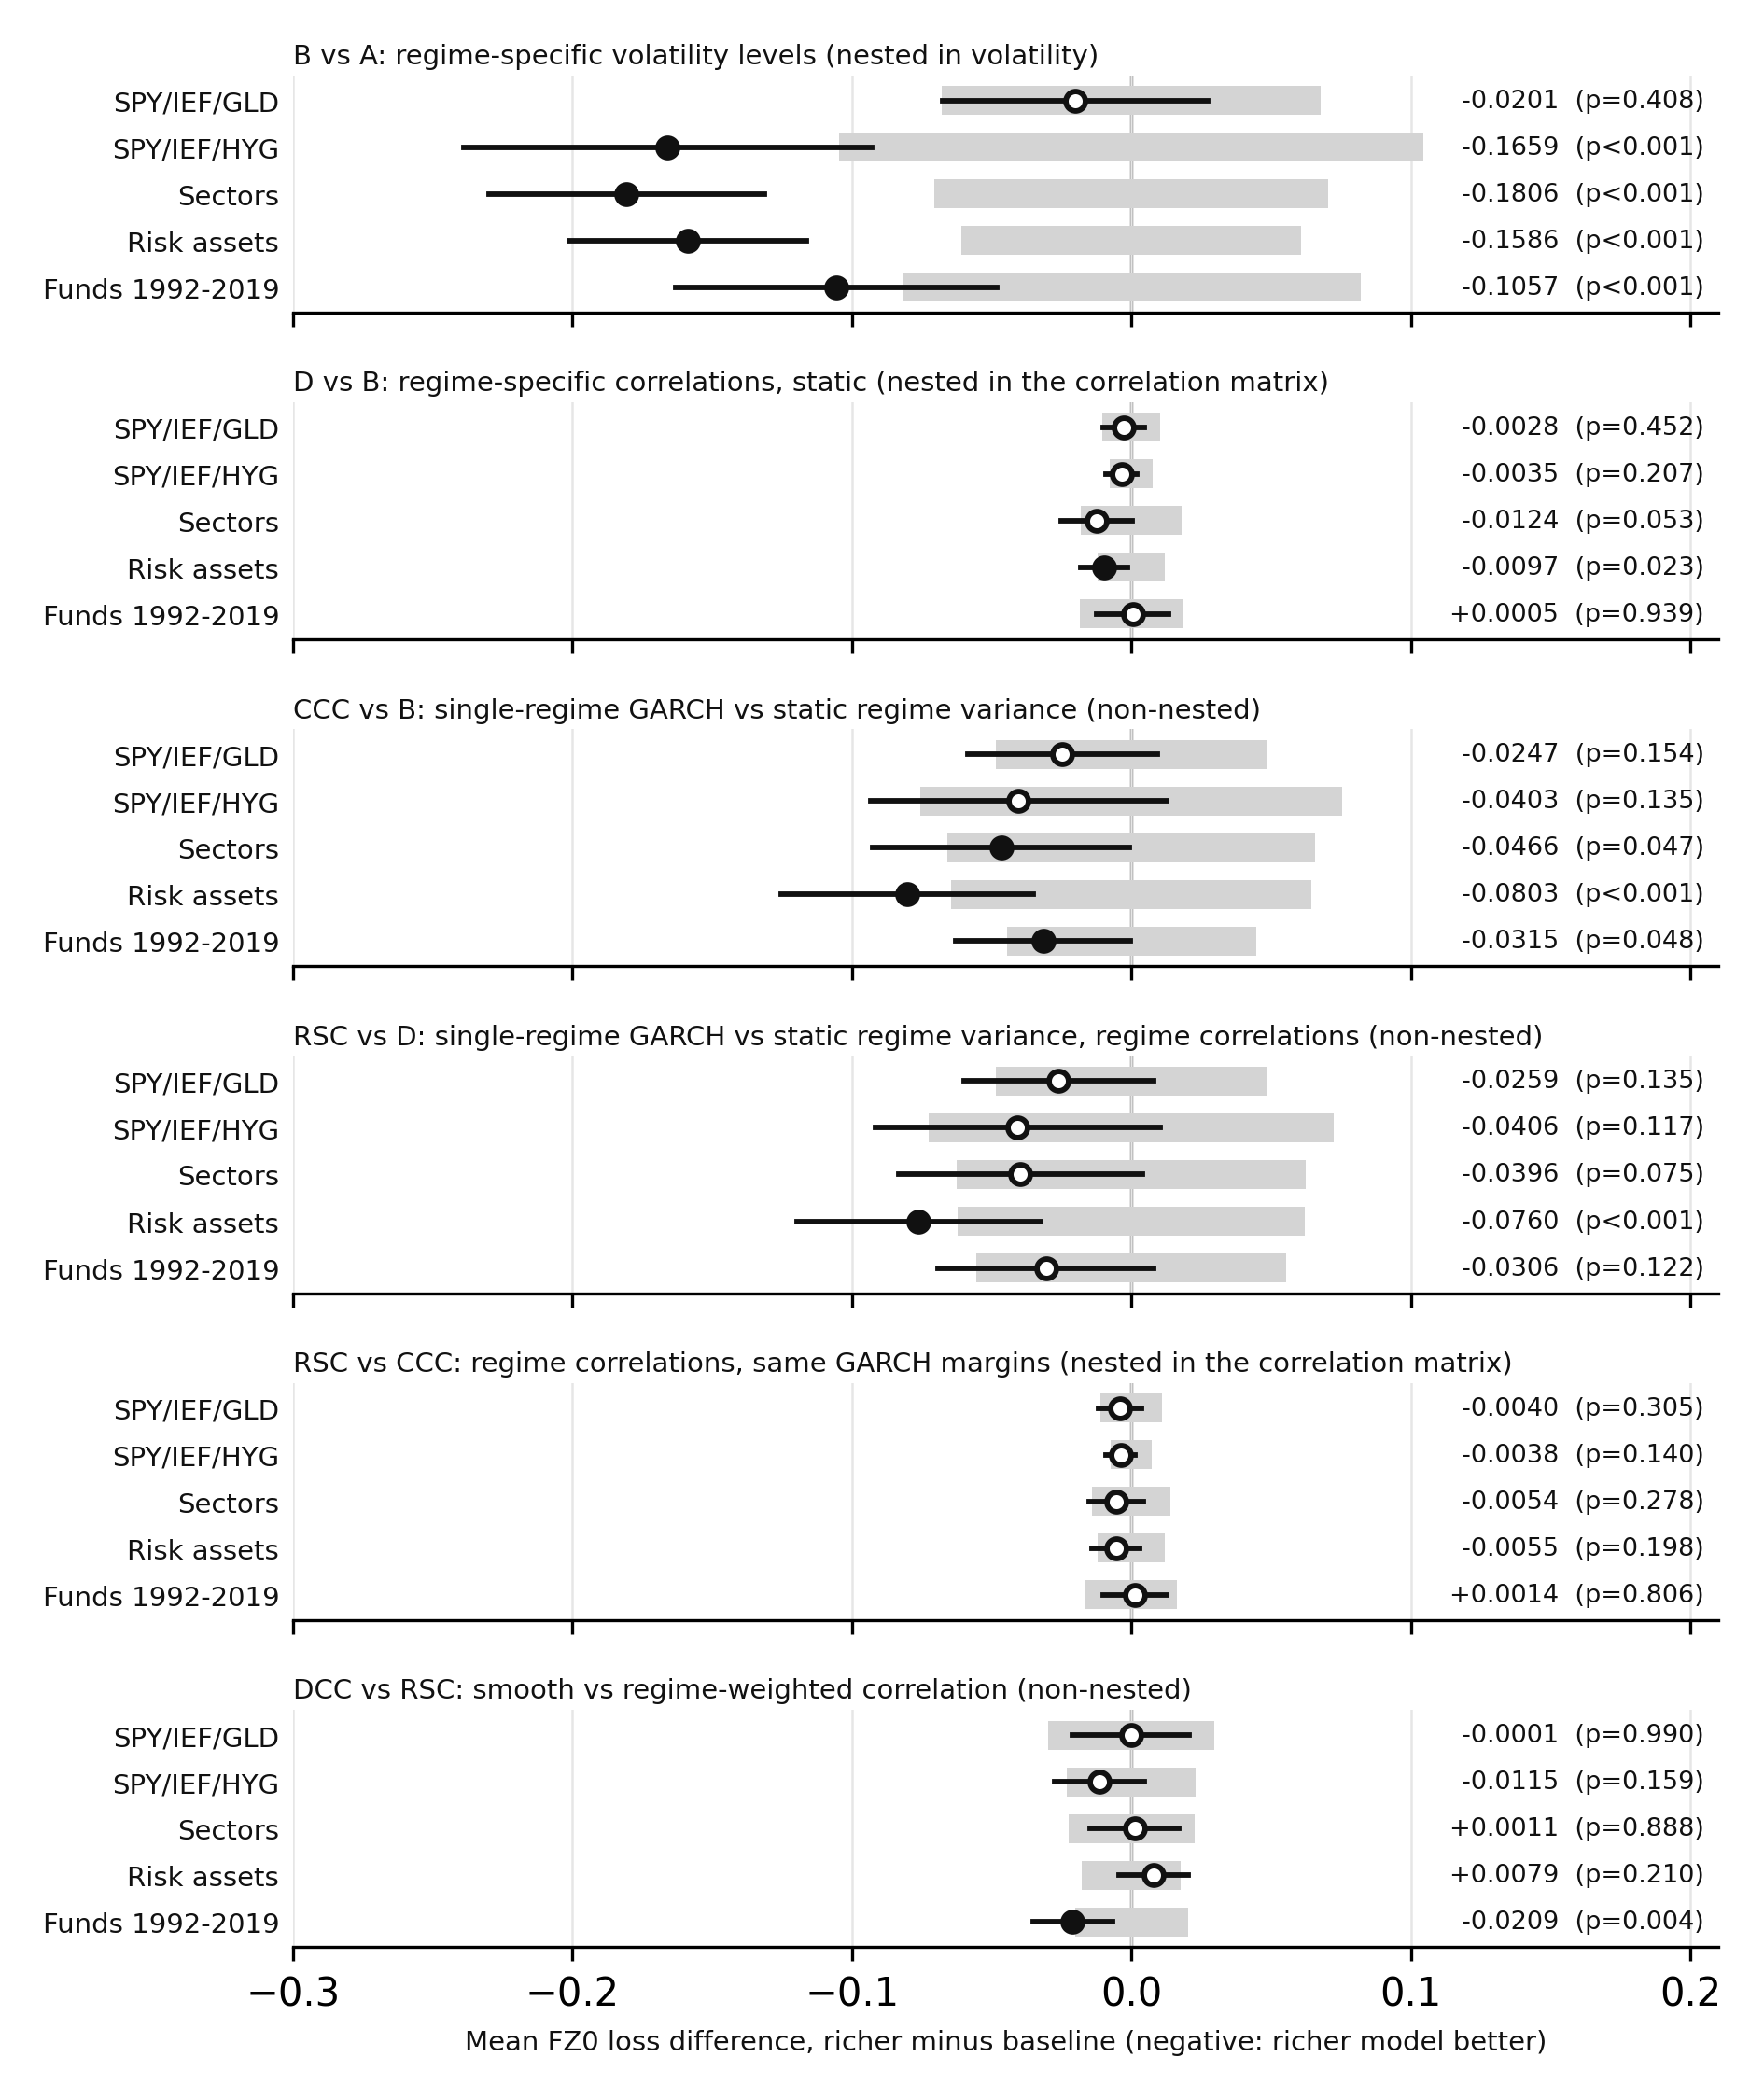
\includegraphics[width=\textwidth,height=0.84\textheight,keepaspectratio]{forest_comparisons_pooled.png}
\caption{\uc{Mean FZ0 difference, richer minus baseline, for each comparison and sample}}\label{fig:forest}
\tabnote{Points are $\bar d$; lines are two-sided 95\% intervals; the grey band is $\pm$ the MDE; filled points have a two-sided $p<0.05$ (unadjusted). Negative favours the richer model. Each panel has its own horizontal scale: the volatility and margin contrasts are roughly ten times larger than the correlation contrasts. Tail level 5\%, Gaussian chain, pooled mean. Source: \texttt{output/explore/ladder/ladder\_dm\_table.csv}, drawn by \texttt{scripts/thesis\_fig\_forest.py}.}
\end{figure}

The size of the contrast depends on the mean treatment, though not its sign. With a zero mean in both models the RSC-versus-D estimates range from $-0.0339$ to $-0.0814$, larger in absolute value than with the pooled mean; with regime-specific means they are close to the pooled ones ($-0.0263$ in the main sample; Appendix~\ref{app:mean}).

Calibration points the same way (Table~\ref{tab:hits}). On the ETF samples the static models overstate risk, with 5\% VaR breached on only 2.8\% to 4.2\% of days for A, B and D, while the GARCH-margin models breach it on 4.3\% to 5.5\%. In the fund sample the static models are close to nominal (B 5.4\%, D 5.3\%).

\begin{table}[t]
\centering\setstretch{1}\footnotesize\setlength{\tabcolsep}{5pt}
\caption{\uc{Share of days on which the return fell below the forecast VaR (nominal 5\%), development data}}\label{tab:hits}
\begin{tabular}{lrrrrrr}
\toprule
Sample & A & B & D & CCC & RSC & DCC \\
\midrule
SPY/IEF/GLD & 3.1\% & 3.7\% & 3.5\% & 5.0\% & 4.7\% & 5.0\% \\
SPY/IEF/HYG & 3.4\% & 4.2\% & 4.0\% & 5.5\% & 5.5\% & 5.0\% \\
Sectors & 3.1\% & 3.4\% & 3.7\% & 5.2\% & 5.4\% & 5.5\% \\
Risk assets & 2.8\% & 2.8\% & 3.0\% & 4.3\% & 4.6\% & 4.7\% \\
Funds 1992--2019 & 4.8\% & 5.4\% & 5.3\% & 5.5\% & 5.2\% & 5.5\% \\
\bottomrule
\end{tabular}
\tabnote{Gaussian chain, pooled mean, forecast days as in Table~\ref{tab:ladder-vol}. A hit is a day with $y_t\le\mathrm{VaR}_t$. Source: \texttt{output/explore/ladder/ladder\_loss\_table.csv}.}
\end{table}


\subsection{The correlation steps}\label{sec:corr-results}

Letting correlations switch, with the volatility model held fixed, never improved the loss detectably (Table~\ref{tab:ladder-corr}). With GARCH margins, switching all correlations (RSC versus CCC) gives estimates between $-0.0040$ and $-0.0055$ in the four ETF samples and $+0.0014$ in the funds; every interval includes zero (two-sided $p$-values from 0.140 to 0.806), and the estimates are between about a third and a half of their MDEs (0.36 to 0.52). The data are consistent with gains up to about the MDE. The answer is not the same under every mean treatment: with a zero mean the sector sample gives $-0.0087$ (two-sided $p=0.046$, unadjusted) and the risk-asset sample $-0.0070$ ($p=0.080$). The smooth alternative, DCC, is indistinguishable from RSC in the ETF samples ($p$ from 0.159 to 0.990) and better than RSC in the fund sample by $0.0209$ ($p=0.004$, unadjusted).

\begin{table}[t]
\centering\setstretch{1}\footnotesize\setlength{\tabcolsep}{5pt}
\caption{\uc{Correlation steps}}\label{tab:ladder-corr}
\begin{tabular}{lrrrcrrr}
\toprule
Sample & $n$ & $\bar d$ & SE & 95\% interval & $t$ & $p$ (2-sided) & MDE \\
\midrule
\multicolumn{8}{l}{\textbf{D versus B (nested in the correlation matrix; size unreliable under GARCH margins)}}\\
SPY/IEF/GLD & 2,516 & $-$0.0028 & 0.0037 & [$-$0.0101, 0.0045] & $-$0.75 & 0.452 & 0.0104 \\
SPY/IEF/HYG & 1,944 & $-$0.0035 & 0.0028 & [$-$0.0089, 0.0019] & $-$1.26 & 0.207 & 0.0078 \\
Sectors & 2,516 & $-$0.0124 & 0.0064 & [$-$0.0249, 0.0002] & $-$1.93 & 0.053 & 0.0179 \\
Risk assets & 1,944 & $-$0.0097 & 0.0043 & [$-$0.0182, $-$0.0013] & $-$2.27 & 0.023 & 0.0120 \\
Funds 1992--2019 & 7,053 & 0.0005 & 0.0066 & [$-$0.0125, 0.0135] & 0.08 & 0.939 & 0.0185 \\
\midrule
\multicolumn{8}{l}{\textbf{RSC versus CCC (nested in the correlation matrix)}}\\
SPY/IEF/GLD & 2,516 & $-$0.0040 & 0.0039 & [$-$0.0117, 0.0037] & $-$1.02 & 0.305 & 0.0110 \\
SPY/IEF/HYG & 1,944 & $-$0.0038 & 0.0026 & [$-$0.0089, 0.0013] & $-$1.48 & 0.140 & 0.0073 \\
Sectors & 2,516 & $-$0.0054 & 0.0050 & [$-$0.0151, 0.0044] & $-$1.08 & 0.278 & 0.0139 \\
Risk assets & 1,944 & $-$0.0055 & 0.0043 & [$-$0.0139, 0.0029] & $-$1.29 & 0.198 & 0.0120 \\
Funds 1992--2019 & 7,053 & 0.0014 & 0.0058 & [$-$0.0099, 0.0128] & 0.25 & 0.806 & 0.0162 \\
\midrule
\multicolumn{8}{l}{\textbf{DCC versus RSC (non-nested)}}\\
SPY/IEF/GLD & 2,516 & $-$0.0001 & 0.0106 & [$-$0.0209, 0.0207] & $-$0.01 & 0.990 & 0.0297 \\
SPY/IEF/HYG & 1,944 & $-$0.0115 & 0.0082 & [$-$0.0276, 0.0045] & $-$1.41 & 0.159 & 0.0229 \\
Sectors & 2,516 & 0.0011 & 0.0081 & [$-$0.0147, 0.0169] & 0.14 & 0.888 & 0.0226 \\
Risk assets & 1,944 & 0.0079 & 0.0063 & [$-$0.0045, 0.0203] & 1.25 & 0.210 & 0.0177 \\
Funds 1992--2019 & 7,053 & $-$0.0209 & 0.0072 & [$-$0.0351, $-$0.0068] & $-$2.90 & 0.004 & 0.0202 \\
\bottomrule
\end{tabular}
\tabnote{As Table~\ref{tab:ladder-vol}.}
\end{table}


The static step D versus B needs a caution. Under the simulated process with GARCH margins and no change in correlation (scenario S0), the one-sided test of D against B rejects in 9.6\% of replications (95\% interval 7.0\% to 12.2\%) at 1,508 test days, in 11.0\% (6.7\% to 15.3\%) at 2,520 days, and in 14.8\% and 17.0\% of replications at $|t|>1.96$ (Table~\ref{tab:power1508}). The test is oversized when volatility clusters. In the exploration grid, 37 of the 214 headline D-versus-B tests have a raw $p<0.05$ (17.3\%), 18 favouring D and 19 favouring B, and none survives a Holm adjustment (smallest adjusted $p=0.1413$). That rate matches the simulated null rate, so the raw count is not evidence of an effect. The simulated process is stylised and the 214 tests are not independent, so the match is suggestive, not proof.

\subsection{The primary pair on the development data}\label{sec:pair-dev}

On the development data the confirmatory comparison, RSC\_P against CCC, gives an estimate of $-0.0015$ over 2010 to 2019 (two-sided $p=0.136$, MDE 0.0028), $-0.0012$ in 2010--2015 ($p=0.371$) and $-0.0019$ in the dry-run years 2016--2019 ($p=0.198$; Table~\ref{tab:real-pair}). These estimates are about the size of the smallest effect of interest and not significant. Their standard errors, $0.0010$, $0.0013$ and $0.0015$, are the ones relevant to the hold-out, which has 1,508 days. Because the pair, the model and the test were chosen with these days in view, they validate nothing.

\begin{table}[t]
\centering\setstretch{1}\footnotesize\setlength{\tabcolsep}{3.5pt}
\caption{\uc{Single-pair correlation switching against constant correlation, development data (RSC\_P versus CCC)}}\label{tab:real-pair}
\begin{tabular}{llrrrcrrr}
\toprule
$\alpha$ & Forecast days & $n$ & $\bar d$ & SE & 95\% interval & $t$ & $p$ (2-sided) & MDE \\
\midrule
5.0\% & 2010--2019 & 2,516 & $-$0.0015 & 0.0010 & [$-$0.0034, 0.0005] & $-$1.49 & 0.136 & 0.0028 \\
5.0\% & 2010--2015 & 1,510 & $-$0.0012 & 0.0013 & [$-$0.0038, 0.0014] & $-$0.89 & 0.371 & 0.0037 \\
5.0\% & 2016--2019 & 1,006 & $-$0.0019 & 0.0015 & [$-$0.0048, 0.0010] & $-$1.29 & 0.198 & 0.0041 \\
2.5\% & 2010--2019 & 2,516 & $-$0.0028 & 0.0015 & [$-$0.0058, 0.0002] & $-$1.82 & 0.069 & 0.0043 \\
2.5\% & 2010--2015 & 1,510 & $-$0.0029 & 0.0021 & [$-$0.0070, 0.0012] & $-$1.37 & 0.171 & 0.0059 \\
2.5\% & 2016--2019 & 1,006 & $-$0.0027 & 0.0022 & [$-$0.0070, 0.0017] & $-$1.20 & 0.231 & 0.0062 \\
\bottomrule
\end{tabular}
\tabnote{RSC\_P minus CCC, Gaussian chain, pooled mean; negative favours switching the SPY--IEF correlation. SE is MDE$/2.8$ (the table stores MDE rounded to $2.8\,\mathrm{SE}$); the interval is $\bar d\pm1.96\,\mathrm{SE}$. These are development data: the specification was chosen after seeing them, so they are not validation. Source: \texttt{output/explore/routes/routes\_dm\_table.csv}, provider HMM\_SPY2.}
\end{table}


\subsection{Power at the hold-out length}\label{sec:power-results}

At 1,508 test days the primary test is correctly sized and has low power (Table~\ref{tab:power1508}). Its size, the rejection rate in S0, is 3.6\% (95\% interval 2.0\% to 5.2\%), so there is no sign of oversizing, although 500 replications cannot show that the size is at most 5\%; the mean difference in S0 is slightly positive, so the null is interior and not on the boundary. The power is 18.2\% (14.8\% to 21.6\%) in the moderate scenario S1, 35.2\% (31.0\% to 39.4\%) in the strong scenario S2 and 2.4\% in the flight-to-quality scenario S3, where correlations move the other way. At 2,520 test days the corresponding one-sided power was 27.0\% and 53.5\%, so the shorter hold-out costs substantial power. The pre-declared low-power rule, which would have made the hold-out chapter open by saying that the test cannot be expected to detect any simulated shift, applied if S2 power fell below 30\%; at 35.2\% it does not apply, but a moderate shift would be detected about one time in five.

\begin{table}[t]
\centering\setstretch{1}\footnotesize\setlength{\tabcolsep}{3.5pt}
\caption{\uc{Simulated size and power of the difference tests (500 replications per scenario at 1,508 days; 200 at 2,520 days)}}\label{tab:power1508}
\begin{tabular}{lcccrr}
\toprule
Scenario & One-sided rejection [95\% CI] & Two-sided & Upper tail & Mean $\bar d$ & Mean SE \\
\midrule
\multicolumn{6}{l}{\textbf{Primary test: RSC\_P versus CCC, 1,508 test days, 500 replications}}\\
S0 (no correlation change) & 3.6\% [2.0\%, 5.2\%] & 7.4\% & 5.2\% & 0.0002 & 0.0006 \\
S1 (moderate) & 18.2\% [14.8\%, 21.6\%] & 14.2\% & 0.4\% & $-$0.0009 & 0.0010 \\
S2 (strong) & 35.2\% [31.0\%, 39.4\%] & 24.2\% & 0.0\% & $-$0.0034 & 0.0026 \\
S3 (flight to quality) & 2.4\% [1.1\%, 3.7\%] & 4.8\% & 3.4\% & 0.0002 & 0.0017 \\
\midrule
\multicolumn{6}{l}{\textbf{Same test, 2,520 test days (earlier study, 200 replications)}}\\
S0 (no correlation change) & 4.5\% [1.6\%, 7.4\%] & 7.0\% & 4.5\% & 0.0001 & 0.0005 \\
S1 (moderate) & 27.0\% [20.8\%, 33.2\%] & 17.5\% & 0.0\% & $-$0.0009 & 0.0008 \\
S2 (strong) & 53.5\% [46.6\%, 60.4\%] & 44.0\% & 0.0\% & $-$0.0035 & 0.0020 \\
S3 (flight to quality) & 5.5\% [2.3\%, 8.7\%] & 3.5\% & 1.0\% & 0.0001 & 0.0013 \\
\midrule
\multicolumn{6}{l}{\textbf{RSC versus CCC (all pairs switch), 1,508 test days}}\\
S0 (no correlation change) & 4.6\% [2.8\%, 6.4\%] & 7.2\% & 4.2\% & 0.0004 & 0.0018 \\
S1 (moderate) & 17.2\% [13.9\%, 20.5\%] & 9.8\% & 0.4\% & $-$0.0022 & 0.0032 \\
S2 (strong) & 25.4\% [21.6\%, 29.2\%] & 17.0\% & 0.0\% & $-$0.0069 & 0.0069 \\
S3 (flight to quality) & 2.6\% [1.2\%, 4.0\%] & 6.6\% & 5.2\% & 0.0010 & 0.0036 \\
\midrule
\multicolumn{6}{l}{\textbf{Static D versus B, 1,508 test days (size under GARCH margins)}}\\
S0 (no correlation change) & 9.6\% [7.0\%, 12.2\%] & 14.8\% & 8.0\% & 0.0002 & 0.0024 \\
\bottomrule
\end{tabular}
\tabnote{Tail level $\alpha=5\%$, Gaussian chain, simulated data from the stylised GARCH regime-switching process (Section~\ref{sec:power-design}); S0 is the null and its row is the test size. One-sided: reject when $t<-1.6449$ (the pre-declared rule). Two-sided: $|t|>1.96$. Upper tail: $t>+1.96$, the rate at which the richer model is declared significantly worse. The interval is a 95\% binomial interval on the replications. Mean $\bar d$ and mean SE are averages over replications. Sources: \texttt{power\_1508\_summary.csv}, \texttt{power\_2520\_twosided.csv}.}
\end{table}


Simulated power does not transfer one-for-one to the real data. The mean standard error of the primary difference in the simulation depends on the scenario: it is 0.0006 in S0, 0.0010 in S1 and 0.0026 in S2, because a larger shift in correlation makes the loss difference more variable. The real-data standard errors above, 0.0010 to 0.0015, lie between the S0 and S2 values, so the power of 35.2\% in S2 reflects both a mean difference of $-0.0034$ and a standard error of 0.0026, and it is not the power that the same difference would have on real data. The minimum detectable difference at the real standard error, about $2.4865\times0.0014=0.0035$ for the one-sided test (0.0031 at the standard error observed on the hold-out, Chapter~\ref{ch:holdout}), is the more transferable summary.

\section{RESULTS: THE HOLD-OUT TEST}\label{ch:holdout}
\todo{Placeholder only. The hold-out (2020-01-02 to 2025-12-31, 1,508 forecast days) has not been run and nothing in this thesis interprets it. After the run this chapter reports the single pre-specified test with the frozen wording of the outcome that occurred (Section~\ref{sec:decision-rule}), simulated power (Table~\ref{tab:power1508}), then the labelled secondary analyses. Anything not pre-registered is marked POST HOC.}

\section{CONTRIBUTIONS, LIMITATIONS AND FUTURE WORK}\label{ch:discussion}

\subsection{Contributions}\label{sec:disc-contrib}

The thesis makes three contributions. First, it evaluates regime-switching correlation for a stock--bond--gold portfolio with a joint VaR--ES loss, which the closest studies do not: \citet{paolella2019} use density and coverage scores on stocks, and \citet{fortin2023} use no regime switching. Second, it separates the volatility, correlation and mean channels under one regime signal. On the development data the gains come from modelling volatility, through regime-specific or GARCH volatility, and not from switching correlations, whose estimates were a third to a half of what the design could detect. Third, it reports a non-significant hold-out result with its interval, minimum detectable difference and power fixed in advance, so that a reader can see which effect sizes the data rule out and which they cannot.

Methodologically, the thesis shows that a common shortcut fails: the static test of regime-specific against pooled correlation is oversized when volatility clusters (Section~\ref{sec:corr-results}), so raw rejection counts across many specifications can look like evidence where there is none. Substantively, the hold-out shows that a desk choosing between these two correlation models is choosing between two forecasts that both under-forecast risk.

\subsection{What the evidence shows and does not show}\label{sec:disc-shows}

The pre-specified test did not reject (outcome O2). The data are consistent with a gain of the size the development data had suggested and with a zero difference, so the result is neither against regime-switching correlation nor for it. Three readings are not supported. That switching fails to improve forecasts: the one-sided lower bound, $-0.0033$, is below the smallest effect of interest of $-0.0020$. That switching helps: the test did not reject, and the 2022 estimate is too imprecise to say anything about the episode that motivated the question. And that the volatility regime, the correlation regime or the GARCH margins is responsible for a particular difference: several comparisons change more than one thing at once (Table~\ref{tab:differs}), and the non-nested ones compare model classes.

The development findings, that regime-specific volatility lowers the loss against a pooled normal, that GARCH margins do better still and that correlation steps are small, rest on many specifications examined after seeing results. I treat them as the reason the thesis has its shape, not as confirmed. The decomposition is the part I would defend most: for each step it gives an estimate, an interval and what the design could detect.

\subsection{What a risk desk should take from the hold-out}\label{sec:disc-calib}

The calibration result is the most useful for a practitioner, although it covers only the two primary models and its explanation is untested. Both breached the 5\% VaR on about 6.9\% of hold-out days, and on breach days losses exceeded the forecast expected shortfall. Which of the two is better is secondary to the fact that both fall short.

The pattern of the evidence points to the level of forecast volatility rather than to the correlation model or the tail shape. The portfolio's volatility rose from 7.1\% a year in the development period to 10.0\% in the hold-out (Table~\ref{tab:data-summary}), the Student-$t$ versions breached more often and not less, and the RiskMetrics EWMA, whose variance adapts within weeks, breached on 5.2\% of days with a loss that cannot be told apart from that of constant correlation. GARCH margins fitted on a five-year window and refitted every 63 days were slower to register the higher level of risk. This explanation fits the evidence but was not tested, and the EWMA comparison was chosen after the result was known. For a portfolio like this one, the evidence gives no reason to adopt regime-switching correlation, and checking the scale of the forecast against recent volatility matters more than the choice of correlation model.

\subsection{Reading the result against the economic framework}\label{sec:disc-slow}

The economic prediction was that, if the stock--bond correlation is driven by equity-market stress, a regime signal built from SPY volatility should help most when the recent correlation is positive. The hold-out does not bear this out. The conditional test did not reject; the favourable loss difference was larger on days with a negative lagged correlation; most of it accrued in 2021, when the calendar-year correlation was $-0.09$; and the switching model lost ground in the 2020 crash, the clearest equity-stress episode in the sample (Figure~\ref{fig:cumulative}). None of this is a test of the two readings, but it sits more easily with the macroeconomic account of \citet{campbell2020} and \citet{molenaar2024}, in which the sign of the correlation follows inflation and real rates and need not coincide with high equity volatility.

Two features of the design would slow any model of this kind. The stress-day correlation is learned from the estimation window, and before 2022 that window held almost no positive stock--bond correlation (Table~\ref{tab:eras}), so the model had little with which to represent a positive stress correlation however quickly the regime moved. And each model is estimated on the last 1,260 days and refitted every 21 days, so in 2022 the correlation changed within a window that still held several years of the old relationship. I did not test either explanation or run a faster-window or different-signal variant on the hold-out, because that analysis was not pre-specified.

\subsection{Limitations}\label{sec:disc-limits}

The following limits apply to every result in the thesis.

\begin{itemize}
\item \textbf{Power.} The test could detect a difference of 0.0031, which exceeds the smallest effect of interest of 0.0020, so outcome O3 required an estimate near or above zero (Section~\ref{sec:sesoi}). The test is better read as a measurement of how precisely this sample can speak than as a test with a realistic chance of excluding a meaningful gain. A longer ETF history would not add the regime of interest (Table~\ref{tab:eras}).
\item \textbf{One test, chosen with the development data in view.} The comparison was selected from a simulation in which the SPY--IEF shift is largest by construction, after I had examined ten universes and ten regime definitions. Nothing was fitted on the hold-out, but the specification is not independent of the exploration, and the pre-registration is a self-registration without an independent timestamp.
\item \textbf{A stylised power study.} The simulated process is an assumption, and simulated and real-data standard errors differ (Section~\ref{sec:power-results}), so the power figures describe the simulated process and need not transfer to markets. The 3.6\% rejection rate in the simulated null (500 replications) is a rough size check, and the upper-tail rate of 8.0\% at 1.645 shows that the normal reference is not exact there.
\item \textbf{Inference.} The estimand is the expected loss difference of two forecasting procedures, each with its own window, refit schedule and hidden-state chain, in the sense of \citet{giacomini2006}; it is not a statement about population parameters. The uncertainty of the estimated regimes is not carried into the test, since I did not bootstrap the whole pipeline. The 2020 and 2021 episodes dominate the average.
\item \textbf{Baselines.} The practitioner baselines, historical simulation and EWMA, were added after the hold-out was scored. They should have been part of the frozen design.
\item \textbf{Signal and window.} The regime signal is the SPY return only, and a volatility signal with a 1,260-day window may be slow to reflect a change in the stock--bond correlation.
\item \textbf{Scope.} There is one portfolio of three funds with constant weights, one data vendor and one reversal episode in the hold-out. The decision is made at the 5\% tail level, chosen for power, while regulatory backtests use the 1\% VaR. I make no claim about other portfolios, tail levels or markets.
\end{itemize}

\subsection{Future work}\label{sec:disc-future}

Each extension below would be a new study with its own pre-specification. A regime signal built from the stock--bond correlation itself or from inflation and real rates would test directly whether a slow macroeconomic state helps where a volatility state did not. A window that adapts to the regime, or exponentially weighted estimates, would address the slowness described above, and the EWMA result suggests that forecast scale should be part of any such comparison. A longer or broader sample, such as several stock--bond portfolios or international funds, would raise the power, and a power calculation like the one in Chapter~\ref{ch:eval} should come first. A bootstrap of the whole estimation pipeline would carry the uncertainty of the regime estimates into the test.

\section{CONCLUSION}\label{ch:conclusion}

I asked whether letting the stock--bond correlation switch with a market regime improves one-day value-at-risk and expected-shortfall forecasts of an equal-weight portfolio of SPY, IEF and GLD. I built a ladder of models that separates the treatment of volatility, correlation and the mean under one regime signal, fixed a single confirmatory test before using 2020--2025, and ran it once.

The test could not tell a gain from none. The estimate favoured switching by 0.0013, the pre-specified test did not reject (outcome O2, Chapter~\ref{ch:holdout}), the sample could not have detected a gain smaller than 0.0031, and a non-significant result is not evidence that the effect is absent.

For a risk manager of a portfolio like this one, the evidence gives no reason to prefer the more complex model, and it does not rule out that the model helps. It also shows a more immediate problem: both primary models breached the 5\% VaR on about 6.8\% to 6.9\% of hold-out days and breach-day losses exceeded the forecast expected shortfall, so neither forecast was well calibrated over 2020--2025. A simple EWMA of the portfolio return, scored post hoc, breached on 5.2\% of days with a loss that cannot be told apart from theirs. On the development data, regime-specific volatility lowered the loss in three of four ETF samples, and the correlation steps were small beside their minimum detectable differences.

The limits are those of Chapter~\ref{ch:discussion}: one portfolio, one vendor, one reversal episode, a regime signal built from equity returns, and a power study that rests on a stylised process. Whether a slower regime signal or a larger sample would show the gain that this one could not is a question for a new, separately pre-specified study.

\section{CODE AND DATA}\label{ch:code}

This chapter explains how the analysis is organised in the accompanying repository, how the data are stored and transformed, and how every table and figure can be reproduced. Paths are relative to the repository root. The code is Python 3.9.6; package versions are pinned in \texttt{requirements.txt}, and the main ones are numpy 2.0.2, pandas 2.3.3, scipy 1.13.1, arch 7.2.0, statsmodels 0.14.6, hmmlearn 0.3.3 and matplotlib 3.9.4.

\subsection{Structure of the repository}\label{sec:code-structure}

\begin{sloppypar}
\begin{description}
\item[\texttt{config/pilot.yaml}] The single source of parameters and seeds: tickers, window (1,260 days), refit intervals (21 and 63 days), tail levels and the simulation design. Its pilot-stage lock date (2016) predates the hold-out design and is not used by the confirmatory run.
\item[\texttt{data/raw/}] The raw Yahoo Finance downloads, never re-pulled, with SHA-256 hashes in \texttt{MANIFEST.txt}. The thesis uses \texttt{spy\_ief\_gld\_raw\_2026-09-26.csv} (main sample) and \texttt{explore\_etfs\_2004\_2019.csv} and \texttt{explore\_rates\_1986\_2019.csv} (development samples). \texttt{data/processed/} and \texttt{data/metadata/} hold pilot-stage files that some tests read.
\item[\texttt{src/}] The models and tests. \texttt{returns.py} builds returns and the portfolio; \texttt{engine.py} holds the hidden Markov model, the mixture VaR and ES, the FZ0 loss, the Diebold--Mariano test and the coverage tests; \texttt{explore\_wf.py} runs the walk-forward forecasts of the static models, DCC and GARCH-$t$; \texttt{explore\_routes.py} runs the GARCH-margin models CCC, RSC and RSC\_P; \texttt{explore\_ladder.py} assembles the ladder; \texttt{explore\_inference.py} implements the Giacomini--White test; \texttt{dgp\_garch.py} simulates the process of the power study.
\item[\texttt{scripts/}] Entry points, in three groups: \texttt{explore\_00} to \texttt{explore\_22} (development results and power studies, Chapter~\ref{ch:results}); \texttt{confirm\_00} to \texttt{confirm\_06} (the frozen hold-out runner and scorer and their checks, Chapter~\ref{ch:holdout}); and \texttt{thesis\_*} together with \texttt{build\_all.py} and \texttt{check\_numbers.py} (tables, figures, post hoc checks and the number trace).
\item[\texttt{output/}] Results: \texttt{explore/} (development), \texttt{confirm/} (dry run, hold-out and post hoc), \texttt{figures/} and \texttt{tables/}.
\item[\texttt{docs/}] The confirmatory specification (\texttt{preregistration\_confirmatory.md}) and the log of every specification tried in development (\texttt{decisions\_log.md}).
\item[\texttt{tests/}] 101 unit tests run by default, and three more that read hold-out-period data and were run only after scoring.
\item[\texttt{thesis/}] The LaTeX source (\texttt{tex/}), the generated tables (\texttt{tex/generated/}), the number registry (\texttt{numbers.yaml}) and the compiled thesis (\texttt{final/thesis.pdf}).
\end{description}
\end{sloppypar}

The files under \texttt{src/}, \texttt{scripts/confirm\_00\_run.py} and \texttt{requirements.txt} are frozen by the tags \texttt{spec-freeze-v1} and \texttt{spec-freeze-v1.1}: the scorer refuses to score forecasts produced by code that differs from the tagged version. Pilot-stage modules in \texttt{src/} therefore remain in place even though no thesis table depends on them.

\subsection{Data storage and transformations}\label{sec:code-data}

The raw file stores every Yahoo field for the three funds from 18 November 2004 to 25 September 2026. The forecasting code reads only the adjusted closes, truncates them at 31 December 2025, drops dates with a missing price, and computes simple returns between consecutive available dates (\texttt{src/returns.py}). The portfolio return is the equal-weighted mean of the three asset returns. Nothing is forward-filled, winsorised or rescaled, except that the GARCH estimation works with returns in per cent and converts back.

Because Yahoo revises adjusted prices when it recomputes distributions, the numbers depend on the data vintage; this is why the raw files are stored with their hashes. A second download of the same three tickers, truncated at 2019, had the same 3,804 dates, and its daily returns differed from the first by at most $2.5\times10^{-6}$ (portfolio returns by at most $9.3\times10^{-7}$). This shows that the download was reproducible across two pulls; it is not a second source, since every ETF series comes from one vendor.

\subsection{Implementation settings}\label{sec:code-settings}

The hidden Markov model is fitted with \texttt{hmmlearn} (diagonal covariance, tolerance $10^{-4}$, seed 0). The first fit of a run is a cold start with 100 iterations from start probabilities $(0.5,0.5)$, a transition matrix with diagonal $(0.98,0.95)$, both means at the window mean, and variances $0.5v$ and $2.5v$, where $v$ is the window variance; every later fit warm-starts from the previous block's estimates with at most 50 iterations. Because the chain carries its estimates forward, a run that starts in 2016 differs slightly from the exploration chain that started in 2010 (a median absolute VaR difference of $1.3\times10^{-5}$ to $1.4\times10^{-5}$ in the primary models); the hold-out run starts cold in the same way.

A regime or hybrid correlation matrix whose smallest eigenvalue is below $10^{-8}$ is repaired by clipping the eigenvalues and rescaling to a unit diagonal. The repair never fired: 0 of 240 matrices in the chain that starts in 2010, 0 of 96 in the chain that starts in 2016, and 0 of 144 in the hold-out run. If a DCC fit returns $\theta_1<0$, $\theta_2<0$ or $\theta_1+\theta_2\ge0.9995$, the code sets $\theta_1=\theta_2=0$; none of the 24 hold-out refits needed this, and no GARCH margin fit failed. BLAS threads are set to one so that the numbers should not depend on the number of cores; I did not test this on another machine.

\subsection{Reproducing the results}\label{sec:code-reproduce}

Table~\ref{tab:reproduce} gives the three levels of reproduction. The quickest rebuilds the thesis from the stored result files; the slowest recomputes everything from the raw data.

\begin{table}[t]
\centering\setstretch{1}\footnotesize
\caption{\uc{How to reproduce the results}}\label{tab:reproduce}
\begin{tabular}{>{\raggedright\arraybackslash}p{4.6cm}>{\raggedright\arraybackslash}p{6.6cm}>{\raggedright\arraybackslash}p{2.4cm}}
\toprule
Task & Command (from the repository root) & Time\\
\midrule
Rebuild all tables and figures, check every registered number, compile the PDF & \texttt{python scripts/build\_all.py} (add \texttt{-{}-no-pdf} to skip LaTeX) & seconds\\
Run the tests & \texttt{python -m pytest -q} & about 1 minute\\
Post hoc checks and baselines & \texttt{python scripts/thesis\_posthoc.py}, \texttt{thesis\_baselines.py} & seconds\\
Dry run and hold-out & \texttt{python scripts/confirm\_00\_run.py pseudo} or \texttt{holdout}, then \texttt{confirm\_01\_score.py} & under 1 minute\\
Development results & \texttt{scripts/explore\_00} to \texttt{explore\_20} in order & several hours\\
Power at the hold-out length & \texttt{scripts/explore\_21\_power\_holdout\_length.py}, then \texttt{explore\_22\_power\_summary.py} & about 19 s per replication, 2,000 replications\\
\bottomrule
\end{tabular}
\tabnote{The hold-out runner refuses to run unless the frozen files match the tag and refuses to overwrite an existing output; the stored hold-out forecasts are \texttt{output/confirm/holdout\_forecasts.pkl}. \texttt{scripts/verify\_clean\_clone.py} repeats the build in a fresh clone and compares each table, figure and the PDF text with the committed versions.}
\end{table}

\texttt{build\_all.py} runs \texttt{thesis\_data\_summary.py}, \texttt{thesis\_tables.py}, \texttt{thesis\_fig\_forest.py}, \texttt{thesis\_fig\_cumulative.py} and \texttt{check\_numbers.py}, then compiles the LaTeX source with \texttt{tectonic}. Every number quoted in the prose that comes from a result file is registered in \texttt{thesis/numbers.yaml} with its source file and format, and \texttt{check\_numbers.py} recomputes each one and checks that it appears in the stated chapter. Table~\ref{tab:exhibits} maps each exhibit to its source.

\begin{table}[t]
\centering\setstretch{1}\scriptsize
\caption{\uc{Source of each table and figure}}\label{tab:exhibits}
\begin{tabular}{>{\raggedright\arraybackslash}p{3.3cm}>{\raggedright\arraybackslash}p{5.4cm}>{\raggedright\arraybackslash}p{4.9cm}}
\toprule
Exhibit & Result file & Produced by\\
\midrule
Tables~\ref{tab:data-summary}, Figure~\ref{fig:corr} & \texttt{output/tables/data\_summary.json} & \texttt{thesis\_data\_summary.py}\\
Table~\ref{tab:eras} & \texttt{output/explore/longhistory\_summary.json} & \texttt{explore\_03\_longhistory.py}\\
Table~\ref{tab:sesoi} & \texttt{output/confirm/sesoi.json} & \texttt{confirm\_04\_sesoi.py}\\
Tables~\ref{tab:ladder-vol}--\ref{tab:ladder-corr}, Figures~\ref{fig:forest}, \ref{fig:forest-zero}, \ref{fig:forest-regime} & \texttt{output/explore/ladder/ladder\_dm\_table.csv}, \texttt{ladder\_loss\_table.csv} & \texttt{explore\_13\_ladder.py}, \texttt{explore\_14\_score\_ladder.py}, \texttt{explore\_15\_longhistory\_ladder.py}\\
Table~\ref{tab:real-pair} & \texttt{output/explore/routes/routes\_dm\_table.csv} & \texttt{explore\_08\_routes.py}, \texttt{explore\_09\_score\_routes.py}\\
Table~\ref{tab:power1508} & \texttt{output/explore/ladder/power\_1508\_summary.csv}, \texttt{power\_2520\_twosided.csv} & \texttt{explore\_16}, \texttt{explore\_20}--\texttt{explore\_22}\\
Tables~\ref{tab:holdout-primary}--\ref{tab:holdout-calib} & \texttt{output/confirm/holdout/*} & \texttt{confirm\_00\_run.py}, \texttt{confirm\_01\_score.py}\\
Figure~\ref{fig:cumulative}, post hoc rows & \texttt{output/confirm/holdout\_forecasts.pkl}, \texttt{posthoc.json}, \texttt{baselines.json} & \texttt{thesis\_fig\_cumulative.py}, \texttt{thesis\_posthoc.py}, \texttt{thesis\_baselines.py}\\
\bottomrule
\end{tabular}
\tabnote{All tables are written to \texttt{thesis/tex/generated/} by \texttt{scripts/thesis\_tables.py}, except Table~\ref{tab:data-summary}, which \texttt{thesis\_data\_summary.py} writes; figures are written to \texttt{output/figures/}. Table~\ref{tab:differs} was derived by hand from the model code.}
\end{table}

\subsection{Checks on the code}\label{sec:code-tests}

The tests check the parts of the pipeline on which the results depend: that no forecast uses information from its own day or later and that dates align across assets; that the FZ0 loss is lower at the true VaR and ES than at biased ones on simulated normal data; that the mixture VaR and ES match their closed forms; that the hidden Markov model recovers known states; the sign convention of $Z_2$ and the Christoffersen test; the scorer's decision rule and validity checks; and the hold-out lock. The scored hold-out tables are listed with their SHA-256 hashes in \texttt{output/confirm/holdout/manifest.json}, and the forecast file has SHA-256 \texttt{9537bb5d6008028076126d0166bb2edc1f643e5a9f496cb852d7872f8485f974}.

\section{Reflection}\label{ch:reflection}

\subsection{From a broad question to a single test}\label{sec:refl-question}

The project began in Phase 1 with a broader question: does a regime-switching covariance model, in which volatilities and correlations both depend on a market state, forecast the tail risk of a stock--bond--gold portfolio better than a single-regime model? The pilot built the static models A to D on SPY, IEF and GLD and judged them against six go/no-go criteria that I wrote down before running them, covering correctness, the size and power of the correlation test, the stability of the estimated regimes, reproducibility and run time. All six passed, but two only narrowly: the power to detect a correlation breakdown reached 50\% only in the strongest simulated scenario, and the regimes were stable in 90.3\% of refits against a 90\% bar. I proceeded with the design, but these margins were the first sign that the correlation question would be hard to answer with daily data on three funds.

My supervisor then asked for a broad exploration of regime definitions and types of ETF. I split the sample so that 2005--2019 would serve for development and 2020--2025 would stay untouched until the test was fixed, and I logged every specification I tried. The exploration changed the question in two ways. First, the static comparison of regime-specific against pooled correlation, which the pilot had judged correctly sized, turned out to be oversized once volatility follows GARCH dynamics, so its many raw rejections were not evidence. This moved the question to models with GARCH margins, where the correlation channel could be isolated with the volatility model held fixed. Second, the long history of fund proxies showed that the development period contains no spell of positive stock--bond correlation, so only the hold-out could speak to the 2022 reversal. The question narrowed from ``do regimes help?'' to one comparison of one correlation, fixed in advance.

\subsection{Challenges and how I addressed them}\label{sec:refl-challenges}

The first challenge was theoretical framing. The literature disagrees about whether the stock--bond correlation follows a slow macroeconomic state or market stress, and my regime signal, built from equity volatility, can speak only to the second. I chose to state this openly as the reading the test addresses rather than to claim more, and Chapter~\ref{ch:discussion} reads the result against both.

The second was methodological. Comparing nested forecasting models out of sample is not covered cleanly by textbook tests, and the papers on the subject treat linear models under squared-error loss. Reading them led me to define the estimand as the expected loss difference of two forecasting procedures, in the sense of Giacomini and White, and to check the size of the test by simulation rather than rely on asymptotic theory. The power study then showed that six years of hold-out data would detect a moderate correlation shift only about one time in five. Rather than look for a more favourable test, I kept the one declared and added a smallest effect of interest and minimum detectable differences, so that a non-significant result would still say something.

The third concerned how results are worded. My supervisor's feedback on an earlier design document cautioned against overstating what each comparison isolates and against reading a non-significant result as evidence of no effect. I corrected that document, built Table~\ref{tab:differs} to state what each comparison changes, and fixed the wording of every possible outcome before the run.

\subsection{What the record shows and what I would change}\label{sec:refl-change}

Two episodes tested the discipline of the design. While searching the test files before the freeze, I displayed two single-day hold-out returns by accident; nothing depended on them, and I disclosed them. And after the hold-out forecasts were produced, the scorer refused them because they had been recorded two commits after the frozen tag, although the forecast code was identical. I amended the check before any number was computed and recorded the change in the specification. Both episodes showed me that a pre-registration kept inside one's own repository is only as credible as the record around it, which is why the appendix sets them out in full.

With hindsight I would change three things. I would include the practitioner baselines, historical simulation and an EWMA, in the frozen design, since the simplest of them turned out to be the best calibrated. I would choose the regime signal from the economic argument, for example from inflation or from the stock--bond correlation itself, rather than from the exploration and the power study. And I would treat calibration as a primary outcome alongside the loss comparison, because for a risk desk it was the more consequential result. What I would keep is the order of work: explore freely, write the test down, then use the hold-out once.


% ---- references and appendices ---------------------------------------------------------------
\clearpage
\begin{singlespace}
\addcontentsline{toc}{section}{REFERENCES}
\bibliography{references}
\end{singlespace}

\clearpage
\appendix
\renewcommand{\thesection}{\Alph{section}}
\titleformat{\section}[block]{\thispagestyle{plain}\centering\normalsize\bfseries}{Appendix \thesection:}{0.5em}{}
\addtocontents{toc}{\protect\renewcommand{\protect\cftsecpresnum}{Appendix~}}
\addtocontents{toc}{\protect\setlength{\protect\cftsecnumwidth}{7.6em}}
\begin{center}\textbf{APPENDIX}\end{center}
\section{SPECIFICATION, REPRODUCIBILITY AND FROZEN WORDING}\label{app:log}

\subsection{Where the record is}

Every methodological decision is in \texttt{docs/decisions\_log.md}, including the exploration grid (10 ETF universes, 10 regime definitions, 214 headline tests) and the family tests. The confirmatory specification is \texttt{docs/preregistration\_confirmatory.md}, fixed by the annotated tags \texttt{spec-freeze-v1} and \texttt{spec-freeze-v1.1}; its section 8 records the one amendment (Section~\ref{sec:holdout-record}). \texttt{docs/EXECUTION\_LOG.md} lists each step of the work in order, with the hashes of the hold-out forecast file and of the scored tables. The hold-out forecast file has SHA-256 \texttt{9537bb5d6008028076126d0166bb2edc1f643e5a9f496cb852d7872f8485f974}; the scored tables are in \texttt{output/confirm/holdout/} with a manifest of their hashes. Tables of the development controls and sub-periods are in \texttt{output/explore/} and are not reprinted.

\subsection{Rebuilding the thesis from saved results}

The command \texttt{python scripts/build\_all.py} rebuilds every table of Chapters 5 to 7, the forest plots and the PDF, and checks every registered number against its source file. It reads the saved result files, refits nothing and takes a few seconds. \texttt{scripts/verify\_clean\_clone.py} repeats the build in a clean clone of the committed repository and compares each table byte for byte, each figure pixel by pixel and the text of the PDF.

\subsection{Recomputing the results}

The saved results can be recomputed from the raw data file stored under \texttt{data/raw/} (SHA-256 \texttt{0ab8c7f3\ldots150e29}) in the order below.
\begin{itemize}
\item The exploration grid, the ladder and the development power study: \texttt{scripts/explore\_00} to \texttt{explore\_20}.
\item Power at the hold-out length: \texttt{scripts/explore\_21\_\allowbreak power\_\allowbreak holdout\_\allowbreak length.py}, 500 replications in each of four scenarios (about 19 seconds per replication), summarised by \texttt{scripts/explore\_22\_power\_summary.py}.
\item The confirmatory dry run and hold-out: \texttt{scripts/confirm\_00\_run.py pseudo} (18 seconds) and \texttt{holdout} (27 seconds), then \texttt{scripts/confirm\_01\_score.py}. The runner refuses to run the hold-out unless the frozen files match the tag and refuses to overwrite an existing output.
\end{itemize}
The test suite (\texttt{pytest}; 105 tests in about one minute, plus three that read the hold-out period) checks the models, the scorer and the helper scripts.

\subsection{Environment}

Python 3.9.6 with numpy 2.0.2, pandas 2.3.3, scipy 1.13.1, arch 7.2.0, statsmodels 0.14.6, hmmlearn 0.3.3 and matplotlib 3.9.4; the full list is in \texttt{requirements.txt}. BLAS threads are set to one so that the numbers should not depend on the core count; I did not test this on another machine.

\subsection{Hidden Markov model initial values}

The first fit of a run is a cold start with 100 iterations from start probabilities $(0.5,0.5)$, a transition matrix with diagonal $(0.98,0.95)$, both means at the window mean, and variances $0.5v$ and $2.5v$, where $v$ is the window variance.

\subsection{Frozen wording of the other outcomes}

The wording fixed before the run for the outcomes that did not occur was:
\begin{description}
\item[O1] ``The hold-out data provide statistical evidence at the one-sided 5\% level that letting the SPY--IEF correlation switch with the regime lowers expected FZ0 loss relative to constant correlation (difference $\bar d$, 95\% CI $[a,b]$). This is one test on one six-year sample containing a single stock--bond reversal; simulated power was $P\%$.''
\item[O3] ``The data are inconsistent, at the one-sided 5\% level, with an improvement larger than SESOI $=0.002$ FZ0 units. Improvements smaller than this, and any degradation, are not excluded.''
\item[O4] ``The hold-out data provide evidence that the switching specification has higher expected FZ0 loss ($\bar d$, 95\% CI $[a,b]$).''
\end{description}


\end{document}
